\section{Hardness result on a grid}
\label{npgrid}
%\todo{maybe we could add a small paragraph somewhere that unit speed rectangular movement area is easy to solve. Andi: i like the idea}
% 

In this section, we study the DDT problem on grid graphs. The grid graph serves as the natural intermediary between a line and a general graph, and they are more closely aligned with applications such as road networks.  Formally, we define a grid graph as follows: The set of vertices is a finite set of integer coordinates $V \subset \mathbb{Z}^2$. 
%For any point with coordinates $x$ and $y$ on the grid, there exists a set of vertices $\{ (a, b)| a,b\in \mathbb{N}, -x \leq a\leq x, -y \leq b\leq y\}$ on the grid. 
An edge of length $1$ connects any two vertices if and only if exactly one of their coordinates differs by exactly one. Therefore we also refer to our grid graph as a \emph{unit grid}. We denote the DDT problem on the unit grid as DDT-Grid. %\todo{simon: can be maybe change this to allow negative coordinates? Andi: i dont see the immediate use of negative coordinates,simon: i use them in my construction. OK, simon: 2 alternatives below}
%For given boundaries $[x_1, x_2]$ and $[y_1, y_2]$ we have the set of vertices $V = \mathbb{Z}^2 \cap [x_1, x_2] \times [y_1, y_2]$.
%For given boundaries $[x_1, x_2]$ and $[y_1, y_2]$ we have a vertex $(x, y) \in \mathbb{Z}^2$ with $x \in [x_1, x_2]$ and $y \in [y_1, y_2]$.




% We will study two cases of DDT problem on grid graphs: the first involves rectangular movement areas with two speeds, discussed in Section~\ref{2grid}, and the second involves arbitrary movement areas with unit speeds in Section~\ref{1grid}. 
% Detailed notations for both cases are provided in the subsequent sections, with Figure~\ref{fig:rectangular_example} offering illustrative examples for each. 

\begin{figure}[ht]
    \centering
    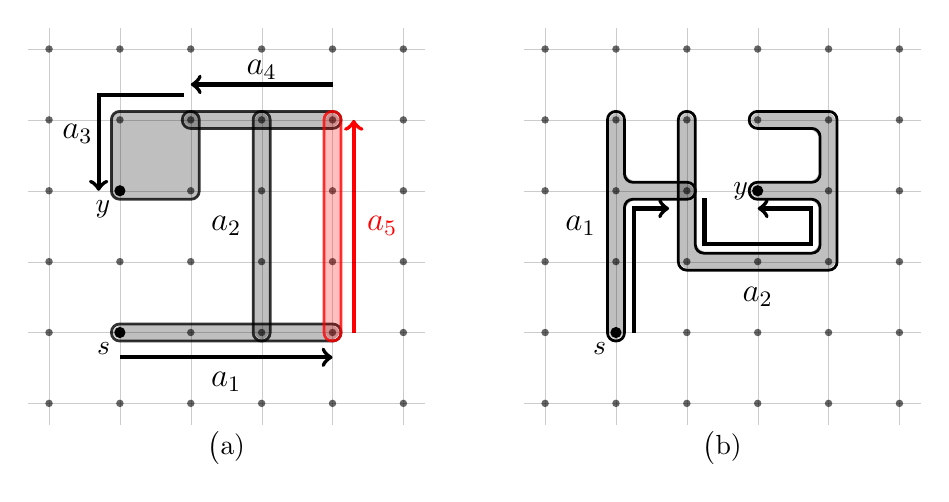
\begin{tikzpicture}[scale=0.9]
\definecolor{b1}{RGB}{0, 0, 0}
\definecolor{b2}{RGB}{4, 75, 145}
\definecolor{b3}{RGB}{76, 68, 194}
\definecolor{b4}{RGB}{50, 140, 190}
\draw[->, line width=1.5] (0, -0.35) -- (3, -0.35);
%\draw[->, dashed, red, line width=1.5] (3.35, 3) -- (3.35, 0);
\draw[<-, red, line width=1.5] (3.3, 3) -- (3.3, 0);
\draw[->, line width=1.5] (3, 3.5000000000000003) -- (1, 3.5000000000000003);
%\draw[<-, dashed, line width=1.5] (3, 3.45) -- (1.1, 3.45);
%\draw[->, dashed, line width=1.5] (1.35, 2) -- (1.35, 2.85);
\draw[->, line width=1.5] (0.9, 3.35) -- (-0.3, 3.35) -- (-0.3, 2);
\def\wi{0.08}
\def\op{0.2}
\def\pts{2.0pt}

\foreach \y in {-1, ...,4} {
\draw[black, line width=\wi, opacity=\op] (-1.3, \y) -- (4.3, \y);
\draw[black, line width=\wi, opacity=\op] (5.7, \y) -- (11.3, \y);
%\draw[black, line width=\wi, opacity=\op] (-46.3, \y) -- (-28.7, \y);
}
\foreach \x in {-1, 0, 1, 2, 3, 4, 6, 7, 8, 9, 10, 11} {
\draw[black, line width=\wi, opacity=\op] (\x, -1.3) -- (\x, 4.3);
%\draw[black, line width=\wi, opacity=\op] (\x, 5.7) -- (\x, 11.3);
%\draw[black, line width=\wi, opacity=\op] (-46.3, \y) -- (-28.7, \y);
}

% \foreach \y in {0,...,23} {
% \draw[black, line width=\wi, opacity=\op] (-25.3, \y) -- (3.3, \y);
% \draw[black, line width=\wi, opacity=\op] (-46.3, \y) -- (-28.7, \y);
% }

\foreach \x in {-1,...,4} {
\foreach \y in {-1,...,4} {
\fill[black, opacity=0.6] (\x, \y) circle (1.5pt);
}
}
\foreach \x in {6,...,11} {
\foreach \y in {-1,...,4} {
\fill[black, opacity=0.6] (\x, \y) circle (1.5pt);
}
}
\draw[b1, line width=1pt, opacity=0.8, rounded corners=3pt] (-0.12, -0.12) rectangle (3.12, 0.12);
\fill[b1, opacity=0.25, rounded corners=5pt] (-0.12, -0.12) rectangle (3.12, 0.12);

\draw[b1, line width=1pt, opacity=0.8, rounded corners=3pt] (1.88, -0.12) rectangle (2.12, 3.12);
\fill[b1, opacity=0.25, rounded corners=5pt] (1.88, -0.12) rectangle (2.12, 3.12);
\draw[b1, line width=1pt, opacity=0.8, rounded corners=3pt] (0.88, 2.88) rectangle (3.12, 3.12);
\fill[b1, opacity=0.25, rounded corners=5pt] (0.88, 2.88) rectangle (3.12, 3.12);
\draw[red, line width=1pt, opacity=0.8, rounded corners=3pt] (2.88, -0.12) rectangle (3.12, 3.12);
\fill[red, opacity=0.25, rounded corners=5pt] (2.88, -0.12) rectangle (3.12, 3.12);
\draw[b1, line width=1pt, opacity=0.8, rounded corners=3pt] (-0.12, 1.88) rectangle (1.12, 3.12);
\fill[b1, opacity=0.25, rounded corners=3pt] (-0.12, 1.88) rectangle (1.12, 3.12);
\draw[black, line width=1pt, rounded corners=3pt](7.88, 3.12) -- (7.88, 0.88) -- (10.120000000000001, 0.88) -- (10.120000000000001, 3.12) -- (8.88, 3.12) -- (8.88, 2.88) -- (9.879999999999999, 2.88) -- (9.879999999999999, 2.12) -- (8.88, 2.12) -- (8.88, 1.88) -- (9.879999999999999, 1.88) -- (9.879999999999999, 1.12) -- (8.12, 1.12) -- (8.12, 3.12) -- cycle;
\fill[black, opacity=0.25, rounded corners=5pt](7.88, 3.12) -- (7.88, 0.88) -- (10.120000000000001, 0.88) -- (10.120000000000001, 3.12) -- (8.88, 3.12) -- (8.88, 2.88) -- (9.879999999999999, 2.88) -- (9.879999999999999, 2.12) -- (8.88, 2.12) -- (8.88, 1.88) -- (9.879999999999999, 1.88) -- (9.879999999999999, 1.12) -- (8.12, 1.12) -- (8.12, 3.12) -- cycle;
\draw[black, line width=1pt, rounded corners=3pt](6.88, -0.12) -- (6.88, 3.12) -- (7.12, 3.12) -- (7.12, 2.12) -- (8.120000000000001, 2.12) -- (8.120000000000001, 1.88) -- (7.12, 1.88) -- (7.12, -0.12) -- cycle;
\fill[black, opacity=0.25, rounded corners=5pt](6.88, -0.12) -- (6.88, 3.12) -- (7.12, 3.12) -- (7.12, 2.12) -- (8.120000000000001, 2.12) -- (8.120000000000001, 1.88) -- (7.12, 1.88) -- (7.12, -0.12) -- cycle;
%\draw[->, dashed, line width=1.5] (6.75, 1) -- (6.75, 0);
\draw[->, line width=1.5] (7.25, 0) -- (7.25, 1.75) -- (7.75, 1.75);
\draw[->, line width=1.5] (8.25, 1.9) -- (8.25, 1.25) -- (9.75, 1.25) -- (9.75, 1.75) -- (9, 1.75);
%\draw[->, dashed, line width=1.5] (8.25, 3) -- (8.25, 2.1);
\filldraw (7, 0) circle (2pt);
\node[below left] at (7, 0) {$s$};
\filldraw (0, 2) circle (2pt);
\node[below left] at (0, 2) {$y$};
\filldraw (9, 2) circle (2pt);
\node[left] at (9, 2) {$y$};
\filldraw (0, 0) circle (2pt);
\node[below left] at (0, 0) {$s$};
% \filldraw[red] (3, 3) circle (2pt);
% \node[above right] at (3, 3) {\textcolor{red}{$p_5$}};
% \filldraw (2, 3) circle (2pt);
\node[] at (9, 0.5) {\large $a_2$};
\node[] at (1.5, 1.5) {\large $a_2$};
\node[] at (1.5, -0.7) {\large $a_1$};
\node[] at (6.5, 1.5) {\large $a_1$};
\node[red] at (3.7, 1.5) {\large $a_5$};
\node[] at (-0.6, 2.8) {\large $a_3$};
\node[] at (2, 3.7) {\large $a_4$};
% \filldraw (1, 2) circle (2pt);
% \node[below right] at (1, 2) {$p_3$};
% \filldraw (1, 3) circle (2pt);
% \node[above right] at (1, 3) {$p_4$};
% \filldraw (0, 3) circle (2pt);
% \node[above left] at (0, 3) {$y$};
% \filldraw (7, 1) circle (2pt);
% \node[above left] at (7, 1) {$p_1$};
% \filldraw (8, 3) circle (2pt);
%\node[above] at (8, 3) {$p_2$};
\node[above] at (1.5, -2) {\big (a)};
\node[above] at (8.5, -2) {\big (b)};
\end{tikzpicture}
%[Finished in 0.2s]
    \caption{Two DDT-Grid instances. On the left is an instance (a) where agents have rectangular movement areas and have two distinct speeds: %On the left, an instance (a) where agents have rectangular movement areas and two speeds:  
    %\simon{
    %  An example of a DDTGR instance with rectangular movement areas different speeds on the left and a DDTG instance with unit speed on the right: In the DDTGR instance, 
    there are four slow agents with speed $1$ and one fast agent with speed $5$, displayed black and red respectively. Each movement area is represented as a rectangle, indicated by shading. 
   % The movement areas represent a rectangle. 
   The optimal solution, with the respective trips indicated by bold solid arrows, takes a total time of $7.6$ by sequentially using agents $a_1 $, $ a_5$, $a_4$ and $ a_3$ to deliver the package from $s$ to $y$. %\andi{ The respective trips are indicated by the bold solid arrows. }
   On the right is an instance (b) with two agents having unit speed, where the movement areas of the agents are not rectangular.
    %On the right is an instance (b) where the movement areas of the agents are not rectangular and there are two agents with speed $1$.
    %On the right, an instance (b) where both movement areas of the drones are not rectangular.
   % In the DDTG instance on the right, 
    %there are two drones with speed $1$, distinguished in the figure by their start points $p_1$ and $p_2$ and their bounded movement subgraphs.  
    Note that even though the nodes of the subgraph of the second agent have rectangular shape, it is not a rectangular movement area as some edges are missing. The optimal solution takes a total time of $8$ by first using agent $a_1$ and then $a_2$ as indicated by the bold solid arrows.}
    \label{fig:rectangular_example}
\end{figure}

We will study the case of DDT-Grid involving agents that are restricted to rectangular movement areas. 
This restriction to rectangular movement areas is natural, reflecting real-world scenarios where agents' movements are typically constrained to specific, license-determined, convex areas, such as road networks.  
Let us define what constitutes a \emph{rectangular} movement area: For every agent $a$, the vertex set $V_a$ forms a rectangular shape, i.e., for every two vertices $x=(x_1,x_2) \in V_a$ and $y=(y_1,y_2)\in V_a$ with $x_1\leq y_1$ and $x_2\leq y_2$, every vertex $z=(z_1,z_2) \in \mathbb{Z}^2$ with $z_1 \in [x_1,y_1]$ and $z_2\in [x_2,y_2]$ must also belong to $V_a$. Regarding $E_a$, for every pair of vertices in $V_a$ differing by exactly 1 in one coordinate, the connecting edge $e$ must be in $E_a$. Intuitively, this ensures that the subgraph forms a rectangle where every possible vertex and edge within that rectangle is included.  This specific scenario will be referred to as DDT-GridR.  
An example of rectangular as well as arbitrary movement areas is given in Figure \ref{fig:rectangular_example}.  

If all agents have the same speed, we can easily provide a polynomial-time algorithm to solve the above DDT-GridR problem without initial positions by constructing the shortest path and generating the corresponding collaborative schedule. However, when agents operate at two different speeds, the problem becomes significantly more complex and challenging.  
We now state the main result regarding this setting. Notice that now unlike in section \ref{npline} we consider the setting of \emph{no initial positioning}. This means we have the flexibility to choose the initial placement of an agent rather than being constrained to fixed starting positions. We refer to the number of vertices $n$ in the grid graph as the \textit{size} of the grid.


\thmgrid*

% \textcolor{blue}{Note that our results from Theorem \ref{thm:line} directly transfer to the case of initial positions. As the movement areas on the line are considered rectangular, we can think of a grid where every agent is positioned on a single grid line. Adapting the construction yields the desired results in the case of fixed starting positions.}

% \andi{I dont think this is actually that easily transferred. The problem I see is that now we have unit grid (or at least equal distance between vertices) and also in the construction there might occur rational values (with the $\frac{1}{P}$ stuff). Maybe we just write that the general ideas could be adapted for the initial position setting if done carefully.}
% \simon{I agree I think it doesn't carry at all, as we use exponential values for the edges in our proof on the Line, which we can't do here as it requires exponential number of node; but maybe this is interesting to write why in our definitions DDT on a path is not a special case of DDT on a grid, because otherwise it may be confusing for reviewers}

 We prove the theorem by showing a reduction from \textsc{2P1N-3SAT}, a special case of \textsc{3SAT}, where each variable in the input formula appears exactly two times as a positive and one time as negative literal. 
 %, and each clause contains at most three literals.  
It is known, that \textsc{2P1N-3SAT} is NP-hard \cite{ryo:2p1nsat}. 
As in Section~\ref{npline}, we will provide a high-level overview of the construction first and later in this section give a formal proof.

%\andi{As previously in section~\ref{npgrid}, due to space limitations we will give a high level overview of the construction in this section. For the detailed construction as well as the complete proof please refer to Appendix~\ref{sec:appendixddtgrapx}.

Let $\phi$, with $n'$ variables and $m'$ clauses, be an instance of the \textsc{2P1N-3SAT} problem. 
The core idea behind the construction of the reduction instance is as follows: For every (of the three) occurrences of each variable we construct an agent which has to make a choice – help with solving the clauses (clause gadgets) or do not help (variable gadgets). Intuitively, the first refers to the literal being set to true, while the latter refers to the literal being set to false in the corresponding assignment.
%Intuitively, the first refers to the literal appearing as positive, while the latter refers to the literal appearing as negative.  
%the first refers to the literal being set to true whereas the latter refers to the literal being set to false.
The design goal of the variable gadgets is to ensure that every assignment is consistent, i.e.\ if $x_i$ is set to true then $\neg x_i$ is set to false. The idea of the clause gadgets is to make sure that the assignment fulfills every clause of the formula. We obtain that the optimal delivery time is below a certain threshold if and only if the given input $\phi$ of \textsc{2P1N-3SAT} is a ``yes''-instance. Furthermore, the DDT-GridR instance is constructed in a way, such that if $\phi$ is not satisfiable, then the additional delivery time increases drastically.


\begin{figure}[h!]
    \centering
    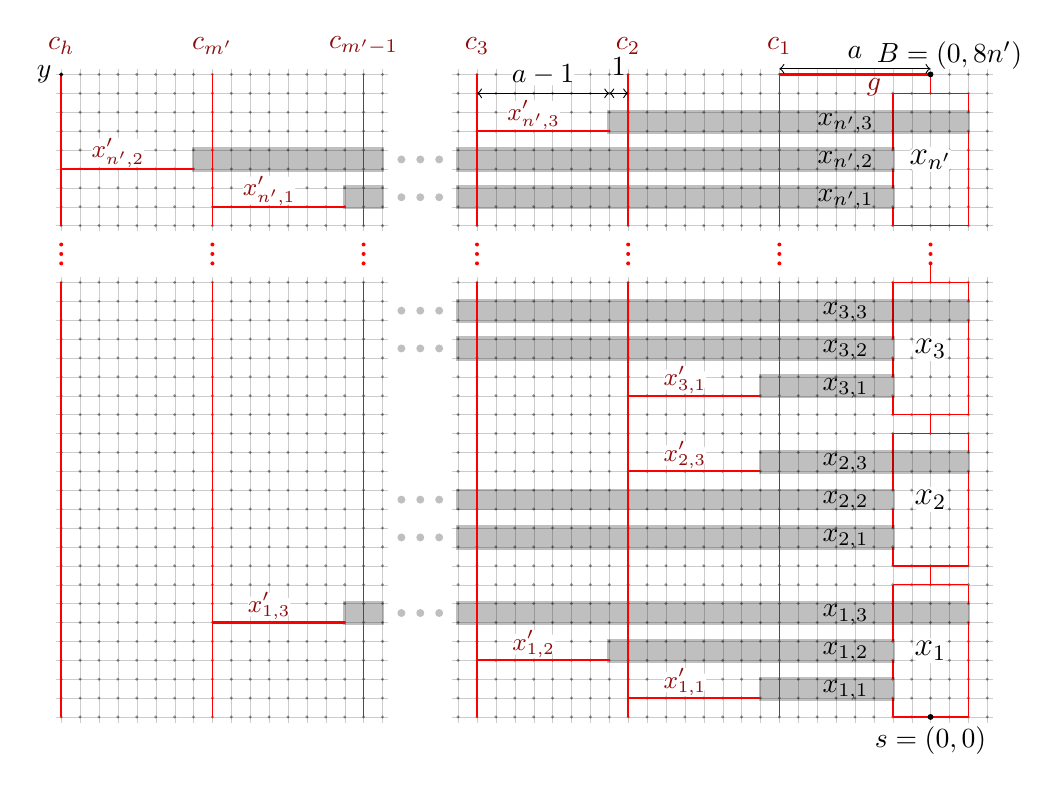
\begin{tikzpicture}[scale=0.24]
\definecolor{dred}{RGB}{143, 11, 11}
\def\wi{0.08}
\def\op{0.2}
\def\pts{2.5pt}

\foreach \x in {-25,...,3} {
\foreach \y in {0,...,23} {
\fill[black, opacity=0.4] (\x, \y) circle (\pts);
}
\draw[black, line width=\wi, opacity=\op] (\x, -0.3) -- (\x, 23.3);
}
\foreach \y in {0,...,23} {
\draw[black, line width=\wi, opacity=\op] (-25.3, \y) -- (3.3, \y);
\draw[black, line width=\wi, opacity=\op] (-46.3, \y) -- (-28.7, \y);
}
\foreach \y in {26,...,34} {
\draw[black, line width=\wi, opacity=\op] (-25.3, \y) -- (3.3, \y);
\draw[black, line width=\wi, opacity=\op] (-46.3, \y) -- (-28.7, \y);
}

\foreach \x in {-25,...,3} {
\foreach \y in {26,...,34} {
\fill[black, opacity=0.4] (\x, \y) circle (\pts);
}
\draw[black, line width=\wi, opacity=\op] (\x, 25.7) -- (\x, 34.3);
}


\foreach \x in {-46,...,-29} {
\foreach \y in {26,...,34} {
\fill[black, opacity=0.4] (\x, \y) circle (\pts);
}
\draw[black, line width=\wi, opacity=\op] (\x, 25.7) -- (\x, 34.3);

}
\foreach \x in {-46,...,-29} {
\foreach \y in {0,...,23} {
\fill[black, opacity=0.4] (\x, \y) circle (\pts);
}
\draw[black, line width=\wi, opacity=\op] (\x, -0.3) -- (\x, 23.3);
}
\draw[red, line width = 0.5669291340000001pt]   (-2, 0) -- (2, 0);
\draw[red, line width = 0.5669291340000001pt]   (-2, 0) -- (-2, 1);
\draw[red, line width = 0.5669291340000001pt]   (-2, 2) -- (-2, 3);
\draw[red, line width = 0.5669291340000001pt]   (-2, 4) -- (-2, 7);
\draw[red, line width = 0.5669291340000001pt]   (2, 0) -- (2, 5);
\draw[red, line width = 0.5669291340000001pt]   (2, 6) -- (2, 7);
\draw[red, line width = 0.5669291340000001pt]   (-2, 7) -- (2, 7);
\draw[red, line width = 0.5669291340000001pt]   (0, 7) -- (0, 8);
\node[fill=white, rounded corners, inner sep=1pt, outer sep=1pt] at (0, 3.5)  {\large $x_1$};
\draw[red, line width = 0.5669291340000001pt]   (-2, 8) -- (2, 8);
\draw[red, line width = 0.5669291340000001pt]   (-2, 8) -- (-2, 9);
\draw[red, line width = 0.5669291340000001pt]   (-2, 10) -- (-2, 11);
\draw[red, line width = 0.5669291340000001pt]   (-2, 12) -- (-2, 15);
\draw[red, line width = 0.5669291340000001pt]   (2, 8) -- (2, 13);
\draw[red, line width = 0.5669291340000001pt]   (2, 14) -- (2, 15);
\draw[red, line width = 0.5669291340000001pt]   (-2, 15) -- (2, 15);
\draw[red, line width = 0.5669291340000001pt]   (0, 15) -- (0, 16);
\node[fill=white, rounded corners, inner sep=1pt, outer sep=1pt] at (0, 11.5)  {\large $x_2$};
\draw[red, line width = 0.5669291340000001pt]   (-2, 16) -- (2, 16);
\draw[red, line width = 0.5669291340000001pt]   (-2, 16) -- (-2, 17);
\draw[red, line width = 0.5669291340000001pt]   (-2, 18) -- (-2, 19);
\draw[red, line width = 0.5669291340000001pt]   (-2, 20) -- (-2, 23);
\draw[red, line width = 0.5669291340000001pt]   (2, 16) -- (2, 21);
\draw[red, line width = 0.5669291340000001pt]   (2, 22) -- (2, 23);
\draw[red, line width = 0.5669291340000001pt]   (-2, 23) -- (2, 23);
\draw[red, line width = 0.5669291340000001pt]   (0, 23) -- (0, 24);
\node[fill=white, rounded corners, inner sep=1pt, outer sep=1pt] at (0, 19.5)  {\large$x_3$};
\draw[red, line width = 0.5669291340000001pt]   (-2, 26) -- (2, 26);
\draw[red, line width = 0.5669291340000001pt]   (-2, 26) -- (-2, 27);
\draw[red, line width = 0.5669291340000001pt]   (-2, 28) -- (-2, 29);
\draw[red, line width = 0.5669291340000001pt]   (-2, 30) -- (-2, 33);
\draw[red, line width = 0.5669291340000001pt]   (2, 26) -- (2, 31);
\draw[red, line width = 0.5669291340000001pt]   (2, 32) -- (2, 33);
\draw[red, line width = 0.5669291340000001pt]   (-2, 33) -- (2, 33);
\draw[red, line width = 0.5669291340000001pt]   (0, 33) -- (0, 34);
\node[fill=white, rounded corners, inner sep=1pt, outer sep=1pt] at (0, 29.5)  {\large $x_{n'}$};
\draw[black, line width = 8.736220474000001pt, opacity=0.25]   (-9.1, 1.5) -- (-1.9, 1.5);
\node at (-4.5, 1.4) { $x_{1, 1}$};
\draw[black, line width = 8.736220474000001pt, opacity=0.25]   (-17.1, 3.5) -- (-1.9, 3.5);
\node at (-4.5, 3.4) { $x_{1, 2}$};
\draw[black, line width = 8.736220474000001pt, opacity=0.25]   (-25.1, 5.5) -- (2.1, 5.5);
\node at (-4.5, 5.4) { $x_{1, 3}$};
\fill[black, opacity=0.25] (-26, 5.5) circle (6pt);
\fill[black, opacity=0.25] (-27, 5.5) circle (6pt);
\fill[black, opacity=0.25] (-28, 5.5) circle (6pt);
\draw[black, line width = 8.736220474000001pt, opacity=0.25]   (-31.1, 5.5) -- (-28.9, 5.5);
\draw[black, line width = 8.736220474000001pt, opacity=0.25]   (-25.1, 9.5) -- (-1.9, 9.5);
\node at (-4.5, 9.4) { $x_{2, 1}$};
\fill[black, opacity=0.25] (-26, 9.5) circle (6pt);
\fill[black, opacity=0.25] (-27, 9.5) circle (6pt);
\fill[black, opacity=0.25] (-28, 9.5) circle (6pt);
\draw[black, line width = 7.836220474000001pt, opacity=0.25]   (-25.1, 11.5) -- (-1.9, 11.5);
\node at (-4.5, 11.4) { $x_{2, 2}$};
\fill[black, opacity=0.25] (-26, 11.5) circle (6pt);
\fill[black, opacity=0.25] (-27, 11.5) circle (6pt);
\fill[black, opacity=0.25] (-28, 11.5) circle (6pt);
\draw[black, line width = 8.736220474000001pt, opacity=0.25]   (-9.1, 13.5) -- (2.1, 13.5);
\node at (-4.5, 13.4) { $x_{2, 3}$};
\draw[black, line width = 8.736220474000001pt, opacity=0.25]   (-9.1, 17.5) -- (-1.9, 17.5);
\node at (-4.5, 17.4) { $x_{3, 1}$};
\draw[black, line width = 8.736220474000001pt, opacity=0.25]   (-25.1, 19.5) -- (-1.9, 19.5);
\node at (-4.5, 19.4) { $x_{3, 2}$};
\fill[black, opacity=0.25] (-26, 19.5) circle (6pt);
\fill[black, opacity=0.25] (-27, 19.5) circle (6pt);
\fill[black, opacity=0.25] (-28, 19.5) circle (6pt);
\draw[black, line width = 8.736220474000001pt, opacity=0.25]   (-25.1, 21.5) -- (2.1, 21.5);
\node at (-4.5, 21.4) { $x_{3, 3}$};
\fill[black, opacity=0.25] (-26, 21.5) circle (6pt);
\fill[black, opacity=0.25] (-27, 21.5) circle (6pt);
\fill[black, opacity=0.25] (-28, 21.5) circle (6pt);
\draw[black, line width = 8.736220474000001pt, opacity=0.25]   (-25.1, 27.5) -- (-1.9, 27.5);
\node at (-4.5, 27.4) { $x_{n', 1}$};
\fill[black, opacity=0.25] (-26, 27.5) circle (6pt);
\fill[black, opacity=0.25] (-27, 27.5) circle (6pt);
\fill[black, opacity=0.25] (-28, 27.5) circle (6pt);
\draw[black, line width = 8.736220474000001pt, opacity=0.25]   (-25.1, 29.5) -- (-1.9, 29.5);
\node at (-4.5, 29.4) { $x_{n', 2}$};
\fill[black, opacity=0.25] (-26, 29.5) circle (6pt);
\fill[black, opacity=0.25] (-27, 29.5) circle (6pt);
\fill[black, opacity=0.25] (-28, 29.5) circle (6pt);
\draw[black, line width = 8.736220474000001pt, opacity=0.25]   (-17.1, 31.5) -- (2.1, 31.5);
\node at (-4.5, 31.4) { $x_{n', 3}$};
% \fill[black, opacity=0.25] (-26, 31.5) circle (6pt);
% \fill[black, opacity=0.25] (-27, 31.5) circle (6pt);
% \fill[black, opacity=0.25] (-28, 31.5) circle (6pt);
\draw[black, line width = 8.736220474000001pt, opacity=0.25]   (-31.1, 27.5) -- (-28.9, 27.5);
\draw[black, line width = 8.736220474000001pt, opacity=0.25]   (-39.1, 29.5) -- (-28.9, 29.5);
\node at (-8, 35.5)  {$\textcolor{dred}{c_1}$};
\draw[red, line width = 0.5669291340000001pt]   (-8, 0) -- (-8, 23);
\draw[red, line width = 0.5669291340000001pt]   (-8, 26) -- (-8, 34);
\fill[red] (-8, 24) circle (3pt);
\fill[red] (-8, 24.5) circle (3pt);
\fill[red] (-8, 25) circle (3pt);
\node at (-16, 35.5)  {$\textcolor{dred}{c_2}$};
\draw[red, line width = 0.5669291340000001pt]   (-16, 0) -- (-16, 23);
\draw[red, line width = 0.5669291340000001pt]   (-16, 26) -- (-16, 34);
\fill[red] (-16, 24) circle (3pt);
\fill[red] (-16, 24.5) circle (3pt);
\fill[red] (-16, 25) circle (3pt);
\node at (-24, 35.5)  {$\textcolor{dred}{c_3}$};
\draw[red, line width = 0.5669291340000001pt]   (-24, 0) -- (-24, 23);
\draw[red, line width = 0.5669291340000001pt]   (-24, 26) -- (-24, 34);
\fill[red] (-24, 24) circle (3pt);
\fill[red] (-24, 24.5) circle (3pt);
\fill[red] (-24, 25) circle (3pt);
\node at (-30, 35.5)  {$\textcolor{dred}{c_{m'-1}}$};
\draw[red, line width = 0.5669291340000001pt]   (-30, 0) -- (-30, 23);
\draw[red, line width = 0.5669291340000001pt]   (-30, 26) -- (-30, 34);
\fill[red] (-30, 24) circle (3pt);
\fill[red] (-30, 24.5) circle (3pt);
\fill[red] (-30, 25) circle (3pt);
\node at (-38, 35.5)  {$\textcolor{dred}{c_{m'}}$};
\draw[red, line width = 0.5669291340000001pt]   (-38, 0) -- (-38, 23);
\draw[red, line width = 0.5669291340000001pt]   (-38, 26) -- (-38, 34);
\fill[red] (-38, 24) circle (3pt);
\fill[red] (-38, 24.5) circle (3pt);
\fill[red] (-38, 25) circle (3pt);
\node at (-46, 35.5)  {$\textcolor{dred}{c_h}$};
\draw[red, line width = 0.5669291340000001pt]   (-46, 0) -- (-46, 23);
\draw[red, line width = 0.5669291340000001pt]   (-46, 26) -- (-46, 34);
\fill[red] (-46, 24) circle (3pt);
\fill[red] (-46, 24.5) circle (3pt);
\fill[red] (-46, 25) circle (3pt);
\fill[red] (0, 24) circle (3pt);
\fill[red] (0, 24.5) circle (3pt);
\fill[red] (0, 25) circle (3pt);
\draw[red, line width = 0.8503937010000002pt]   (-8, 34) -- (0, 34);
\draw[red, line width = 0.8503937010000002pt]   (-16, 1) -- (-9, 1);
\node[fill=white, rounded corners, inner sep=0pt, outer sep=0pt] at (-13, 1.85) { \small $\textcolor{dred}{x_{1, 1}'}$};
\draw[red, line width = 0.8503937010000002pt]   (-16, 13) -- (-9, 13);
\node[fill=white, rounded corners, inner sep=0pt, outer sep=0pt] at (-13, 13.85) { \small $\textcolor{dred}{x_{2, 3}'}$};
\draw[red, line width = 0.8503937010000002pt]   (-16, 17) -- (-9, 17);
\node[fill=white, rounded corners, inner sep=0pt, outer sep=0pt] at (-13, 17.85) { \small $\textcolor{dred}{x_{3, 1}'}$};
\draw[red, line width = 0.8503937010000002pt]   (-24, 3) -- (-17, 3);
\node[fill=white, rounded corners, inner sep=0pt, outer sep=0pt] at (-21, 3.85) { \small $\textcolor{dred}{x_{1, 2}'}$};
\draw[red, line width = 0.8503937010000002pt]   (-24, 31) -- (-17, 31);
\node[fill=white, rounded corners, inner sep=0pt, outer sep=0pt] at (-21, 31.85) { \small $\textcolor{dred}{x_{n', 3}'}$};
\draw[red, line width = 0.8503937010000002pt]   (-38, 5) -- (-31, 5);
\node[fill=white, rounded corners, inner sep=0pt, outer sep=0pt] at (-35, 5.85) { \small $\textcolor{dred}{x_{1, 3}'}$};
\draw[red, line width = 0.8503937010000002pt]   (-38, 27) -- (-31, 27);
\node[fill=white, rounded corners, inner sep=0pt, outer sep=0pt] at (-35, 27.85) { \small $\textcolor{dred}{x_{n', 1}'}$};
\draw[red, line width = 0.8503937010000002pt]   (-46, 29) -- (-39, 29);
\node[fill=white, rounded corners, inner sep=0pt, outer sep=0pt] at (-43, 29.85) { \small $\textcolor{dred}{x_{n', 2}'}$};
%\filldraw (0, -4) circle (2pt);
%\node[left] at (0, -4) {$s=(0, - n^5)$};
\filldraw (0, 0) circle (3.5pt);
\node[below] at (0, 0) {$s = (0, 0)$};
\filldraw (0, 34) circle (3.5pt);
\node[] at (1, 35) {$B = (0, 8n')$};
\filldraw (-46, 34) circle (2pt);
\node[left] at (-46, 34) {$y$};
\draw[<->] (-24, 33) -- (-17, 33) node[midway, above=3pt, fill=white, rounded corners, inner sep=0pt, outer sep=0pt] {$a-1$};
\draw[<->] (-17, 33) -- (-16, 33) node[midway, above=3pt] {$1$};
\draw[<->] (-8, 34.3) -- (0, 34.3) node[midway, above] {$a$};
%\draw[black, line width = 0.5669291340000001pt]   (0, 0) -- (0, -4);
%\node[left] at (0, -2)  {$d$};
\node[fill=white, rounded corners, inner sep=0pt, outer sep=0pt] at (-3, 33.3) {$\textcolor{dred}{g}$};
%\node[fill=white, rounded corners] at (0, 0) {$s$};
\end{tikzpicture}
%[Finished in 0.1s]
    \caption{A sketch of the DDT-GridR instance: The package is to be delivered from the bottom-right to the top-left.  The grey bars represent the rectangular movement areas of the literal agents associated with the three occurrences of every variable (two positive $x_{i,1},x_{i,2}$, as well as one negative $x_{i,3}$ ). On the left side we have $m'$ clause gadgets. In this example clause $c_1$ contains literals $x_1$, $\neg x_2$, and $x_3$. Therefore we have the three agents $x'_{1,1},x'_{2,3},x'_{3,1}$, which work as counterparts to $x_{1,1},x_{2,3},x_{3,1}$ delivering the package between two clause gadgets. Agent $c_h$ (on the far left)  serves as an auxiliary agent to assist with the delivery to $y$. On the right side we have $n'$ variable gadgets. Every optimal schedule (given $\phi$ is satisfiable) must traverse all variable gadgets up to point $B$, as delivering horizontally over a distance $a$ with a slow agent would require an excessive amount of time.}
\label{fig:grid_2speed}
\end{figure}

Let us begin to construct the resulting instance for DDT-GridR. For a complete overview see Figure \ref{fig:grid_2speed}. The two different speeds are depicted in red (fast) and grey (slow). Note that every single straight red line represents a fast agent and we want to deliver the package from bottom right ($s$) to top left ($y$). 
For every occurrence of each variable $x_i$ we construct agents $x_{i,1},x_{i,2}$ and $x_{i,3}$ where each of the first two corresponds to one of the positive occurrences and the latter one corresponds to the negative occurrence $\neg x_i$. We will refer to these as the \textit{literal agents}. 
As briefly mentioned before, all literal agents referring to $x_i$ can now contribute to our schedule either in a clause gadget containing $x_i$ or $\neg x_i$, or in the variable gadget corresponding to $x_i$. More precisely, each of $x_{i,1}$ and $x_{i,2}$ have a distinct clause gadget assigned such that the clause contains literal $x_i$ and $x_{i,3}$ has the clause gadget assigned that has the unique occurrence of $\neg x_i$. From Figure \ref{fig:grid_2speed} we observe that the presence of a (slow) literal agent $x_{i,k}$ in clause $c_j$ is required to fill the gap of length 1 (left of the fast agent labeled with $c_j$) to deliver to the fast agent $x'_{i,k}$. We can think of filling this gap as satisfying the particular clause. 

We have discussed the inclusion of both the clause gadget and the variable gadget in the instance construction. First, let us take a closer look at the variable gadgets depicted on the right side of Figure \ref{fig:grid_2speed}. The design goal of the variable gadget is to ensure feasible assignments, that is, either $x_i$ or $\neg x_i$ – but not both – contributes to solving the clauses and is
%does not contribute to solving the clauses or in other words is 
set to true. A close-up on a variable gadget is given by Figure \ref{fig:grid_var_gadget}. Note that this is just one of all $n'$ consecutive variable gadgets and each gadget consists of multiple fast agents (every straight red line). For the traversal of a variable gadget from bottom to top, either both positive literal agents or the negative literal agent have to engage with it. If the traversal starts at $s$, passes through all consecutive variable gadgets, and finishes at
$B$ (see Fig~\ref{fig:grid_2speed}), we can infer that literal agents were placed to help carry the package across the gaps (two gaps on the left side or one gap on the right side of each variable gadget). 
%If starting from $s$ all consecutive variable gadgets are traversed finishing in $B$ (see Fig~\ref{fig:grid_2speed}), we know that there were literal agents placed to help carry the package over the gaps.   

%We can think of these literals being set to false. 

As we move toward the clause gadgets (utilizing auxiliary agent $g$) we run into the following situation: To assist in traversing the gaps induced by the clause gadgets, we can only incorporate the  %previously unused 
literal agents that were not placed in the variable gadget. If we rely on a literal agent that was already placed on the right side of the instance, helping in the variable gadget, to also carry over a gap of a clause gadget,
we know that this agent has traveled at least a certain distance, $a$, at a slow speed.
%we know that this agent traveled distance at least $a$ with slow speed. 
Setting $a$ to be sufficiently large, we can conclude that a schedule utilizing a literal agent in the variable gadget as well as a clause gadget is too slow to beat a threshold time $t$ which assumes that all gaps can be traversed by distinct literal agents. The same holds for using a literal agent in multiple clause gadgets as they also have a horizontal distance of $a$. It is especially important, that the speed of the fast agents depends on $a$ and $a$ itself is relying on $n'$ and $\varepsilon$. 
Essentially, setting $a$ sufficiently large ensures that traveling a distance of $a$ at a slow speed results in a delivery time that is more than  
%large enough ensures that travelling distance $a$ with slow speed makes the delivery time more than  
$n^{1-\varepsilon}$ (with $n$ being the size of the grid) times as large as the delivery time for a satisfiable instance of \textsc{2P1N-3SAT} (using the satisfying assignment in the clause gadgets and the complements in the variable gadgets).

Finally, we get to the essence of the reduction proof argument: 
%Finally we get to the   the essence of the reduction proof argument:  
If there exists a feasible assignment ($\phi$ is a ``yes''-instance), then we can place the agents in a way such that no literal agent has to bridge more than a single gap and the optimal delivery time must be within the threshold. Consequently, the delivery time of an $n^{1-\varepsilon}$-approximation algorithm must be within $n^{1-\varepsilon}$ times the threshold; On the other hand, if we have a sufficiently fast delivery schedule, we can rebuild the assignment by looking at the literal agents placed in the variable gadgets and output (the inverse) as a feasible solution. If the delivery time of the approximation algorithm is less than $n^{1-\varepsilon}$ times the threshold, it is impossible for a slow agent to have traveled a horizontal distance of $a$, as this would take more than $n^{1-\varepsilon}$ times the threshold. This ensures a feasible and satisfying assignment, therefore $\phi$ is a ``yes''-instance. 

%If the delivery time of an $n^{1-\varepsilon}$-approximation algorithm exceeds $n^{1-\varepsilon}$ times the threshold, then the optimal delivery time must also exceed the threshold, therefore $\phi$ is a 'no'-instance. 
%If $\phi$ is a ``yes''-instance, the optimal delivery time must be within the threshold. Consequently, the delivery time of an $n^{1-\varepsilon}$-approximation algorithm must be within $n^{1-\varepsilon}$ times the threshold. Conversely, if the delivery time of the approximation algorithm is less than $n^{1-\varepsilon}$ times the threshold, it is impossible for a slow agent to have traveled a horizontal distance of $a$, as this would take more than $n^{1-\varepsilon}$ times the threshold. This ensures a feasible and satisfying assignment, therefore $\phi$ is a ``yes''-instance.


\begin{figure}[ht]
    \centering
    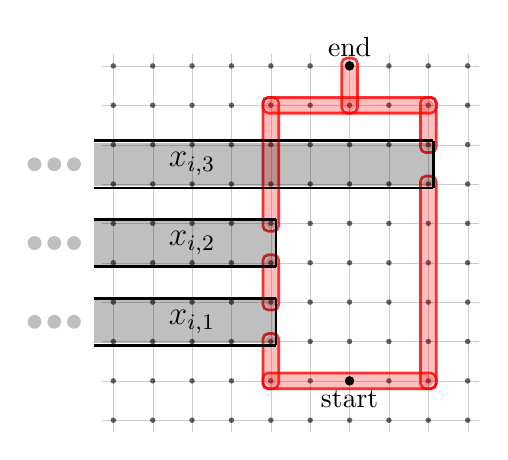
\begin{tikzpicture}[scale=0.50]
\def\wi{0.08}
\def\op{0.2}
\def\pts{2.0pt}
\foreach \x in {-6,...,3} {
\foreach \y in {-1,...,8} {
\fill[black, opacity=0.6] (\x, \y) circle (\pts);
}
}

\foreach \x in {-6,...,3} {
\draw[black, line width = \wi, opacity=\op] (\x, -1.3) -- (\x, 8.3);
}
\foreach \y in {-1,...,8} {
    \draw[black, line width = \wi, opacity=\op] (-6.3,  \y) -- (3.3, \y);

}
%\draw[red, line width = 2.267716536pt]   (-2, 0) -- (2, 0);
\draw[red, line width=1pt, opacity=0.8, rounded corners=2pt] (-2.2, -0.2) rectangle (2.2, 0.2);
\fill[red, opacity=0.25, rounded corners=5pt] (-2.2, -0.2) rectangle (2.2, 0.2);

%\draw[red, line width = 2.267716536pt]   (-2, 0) -- (-2, 1);

\draw[red, line width=1pt, opacity=0.8, rounded corners=2pt] (-2.2, -0.2) rectangle (-1.8, 1.2);
\fill[red, opacity=0.25, rounded corners=5pt] (-2.2, -0.2) rectangle (-1.8, 1.2);

% \draw[red, line width = 2.267716536pt]   (-2, 2) -- (-2, 3);

\draw[red, line width=1pt, opacity=0.8, rounded corners=2pt] (-2.2, 1.8) rectangle (-1.8, 3.2);
\fill[red, opacity=0.25, rounded corners=5pt] (-2.2, 1.8) rectangle (-1.8, 3.2);

% \draw[red, line width = 2.267716536pt]   (-2, 4) -- (-2, 7);


\draw[red, line width=1pt, opacity=0.8, rounded corners=2pt] (-2.2, 3.8) rectangle (-1.8, 7.2);
\fill[red, opacity=0.25, rounded corners=5pt] (-2.2, 3.8) rectangle (-1.8, 7.2);


% \draw[red, line width = 2.267716536pt]   (2, 0) -- (2, 5);


\draw[red, line width=1pt, opacity=0.8, rounded corners=2pt] (1.8, -0.2) rectangle (2.2, 5.2);
\fill[red, opacity=0.25, rounded corners=5pt] (1.8, -0.2) rectangle (2.2, 5.2);

%\draw[red, line width = 2.267716536pt]   (2, 6) -- (2, 7);


\draw[red, line width=1pt, opacity=0.8, rounded corners=2pt] (1.8, 5.8) rectangle (2.2, 7.2);
\fill[red, opacity=0.25, rounded corners=5pt] (1.8, 5.8) rectangle (2.2, 7.2);


%\draw[red, line width = 2.267716536pt]   (-2, 7) -- (2, 7);
\draw[red, line width=1pt, opacity=0.8, rounded corners=2pt] (-2.2, 6.8) rectangle (2.2, 7.2);
\fill[red, opacity=0.25, rounded corners=5pt] (-2.2, 6.8) rectangle (2.2, 7.2);

%\draw[red, line width = 2.267716536pt]   (0, 7) -- (0, 8);
\draw[red, line width=1pt, opacity=0.8, rounded corners=2pt] (-0.2, 6.8) rectangle (0.2, 8.2);
\fill[red, opacity=0.25, rounded corners=5pt] (-0.2, 6.8) rectangle (0.2, 8.2);

\filldraw (0, 0) circle (3pt);
\node[below] at (0, 0) {start};
\filldraw (0, 8) circle (3pt);
\node[above] at (0, 8) {end};
%\draw[red, line width=1pt, opacity=0.8, rounded corners=2pt] (-0.2, 6.8) rectangle (0.2, 8.2);
\draw[black, line width = 1pt]   (-6.5, 2.1) -- (-1.87, 2.1);
\draw[black, line width = 1pt]   (-6.5, 0.9) -- (-1.87, 0.9);
\draw[black, line width = 1pt]   (-1.87, 2.1) -- (-1.87, 0.9);
\draw[black, line width = 1pt]   (-6.5, 4.1) -- (-1.87, 4.1);
\draw[black, line width = 1pt]   (-6.5, 2.9) -- (-1.87, 2.9);
\draw[black, line width = 1pt]   (-1.87, 4.1) -- (-1.87, 2.9);
\draw[black, line width = 1pt]   (-6.5, 6.1) -- (2.13, 6.1);
\draw[black, line width = 1pt]   (-6.5, 4.9) -- (2.13, 4.9);
\draw[black, line width = 1pt]   (2.13, 6.1) -- (2.13, 4.9);
\draw[black, opacity=0.25, line width = 15.590551185000002pt]   (-6.5, 1.5) -- (-1.87, 1.5);
\draw[black, opacity=0.25, line width = 15.590551185000002pt]   (-6.5, 3.5) -- (-1.87, 3.5);
\draw[black, opacity=0.25, line width = 15.590551185000002pt]   (-6.5, 5.5) -- (2.13, 5.5);
\fill[black, opacity=0.25] (-7, 1.5) circle (5pt);
\fill[black, opacity=0.25] (-7.5, 1.5) circle (5pt);
\fill[black, opacity=0.25] (-8, 1.5) circle (5pt);
\node at (-4, 1.5) { \large $x_{i, 1}$};
\fill[black, opacity=0.25] (-7, 3.5) circle (5pt);
\fill[black, opacity=0.25] (-7.5, 3.5) circle (5pt);
\fill[black, opacity=0.25] (-8, 3.5) circle (5pt);
\node at (-4, 3.5) { \large $x_{i, 2}$};
\fill[black, opacity=0.25] (-7, 5.5) circle (5pt);
\fill[black, opacity=0.25] (-7.5, 5.5) circle (5pt);
\fill[black, opacity=0.25] (-8, 5.5) circle (5pt);
\node at (-4, 5.5) { \large $x_{i, 3}$};
\end{tikzpicture}
%[Finished in 0.2s]
    \caption{Depiction of the variable gadget of $x_i$. It consists of 8 fast agents (red). To deliver the package from ``start'' to ``end'', it must traverse either the left or right side of the gadget. For the left side, both $x_{i, 1}$ and $x_{i, 2}$ must be present to deliver the package across the two gaps; while for the right side, only $x_{i, 3}$ is required to cover a single gap. 
    Note that skipping the gadget and traversing the distance $a$ horizontally using a literal agent is too slow and therefore not feasible for satisfiable inputs.}
    %Note that skipping the gadget and traversing distance $a$ horizontally via some literal agent is too slow and will not be feasible for satisfiable inputs.}}
    \label{fig:grid_var_gadget}
\end{figure}

% \begin{figure}[h!]
%     \centering
%     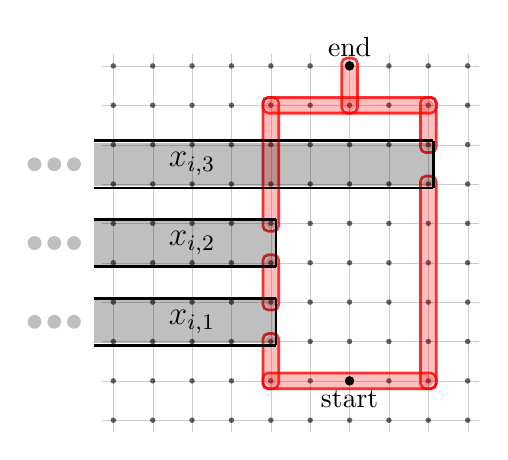
\begin{tikzpicture}[scale=0.50]
\def\wi{0.08}
\def\op{0.2}
\def\pts{2.0pt}
\foreach \x in {-6,...,3} {
\foreach \y in {-1,...,8} {
\fill[black, opacity=0.6] (\x, \y) circle (\pts);
}
}

\foreach \x in {-6,...,3} {
\draw[black, line width = \wi, opacity=\op] (\x, -1.3) -- (\x, 8.3);
}
\foreach \y in {-1,...,8} {
    \draw[black, line width = \wi, opacity=\op] (-6.3,  \y) -- (3.3, \y);

}
%\draw[red, line width = 2.267716536pt]   (-2, 0) -- (2, 0);
\draw[red, line width=1pt, opacity=0.8, rounded corners=2pt] (-2.2, -0.2) rectangle (2.2, 0.2);
\fill[red, opacity=0.25, rounded corners=5pt] (-2.2, -0.2) rectangle (2.2, 0.2);

%\draw[red, line width = 2.267716536pt]   (-2, 0) -- (-2, 1);

\draw[red, line width=1pt, opacity=0.8, rounded corners=2pt] (-2.2, -0.2) rectangle (-1.8, 1.2);
\fill[red, opacity=0.25, rounded corners=5pt] (-2.2, -0.2) rectangle (-1.8, 1.2);

% \draw[red, line width = 2.267716536pt]   (-2, 2) -- (-2, 3);

\draw[red, line width=1pt, opacity=0.8, rounded corners=2pt] (-2.2, 1.8) rectangle (-1.8, 3.2);
\fill[red, opacity=0.25, rounded corners=5pt] (-2.2, 1.8) rectangle (-1.8, 3.2);

% \draw[red, line width = 2.267716536pt]   (-2, 4) -- (-2, 7);


\draw[red, line width=1pt, opacity=0.8, rounded corners=2pt] (-2.2, 3.8) rectangle (-1.8, 7.2);
\fill[red, opacity=0.25, rounded corners=5pt] (-2.2, 3.8) rectangle (-1.8, 7.2);


% \draw[red, line width = 2.267716536pt]   (2, 0) -- (2, 5);


\draw[red, line width=1pt, opacity=0.8, rounded corners=2pt] (1.8, -0.2) rectangle (2.2, 5.2);
\fill[red, opacity=0.25, rounded corners=5pt] (1.8, -0.2) rectangle (2.2, 5.2);

%\draw[red, line width = 2.267716536pt]   (2, 6) -- (2, 7);


\draw[red, line width=1pt, opacity=0.8, rounded corners=2pt] (1.8, 5.8) rectangle (2.2, 7.2);
\fill[red, opacity=0.25, rounded corners=5pt] (1.8, 5.8) rectangle (2.2, 7.2);


%\draw[red, line width = 2.267716536pt]   (-2, 7) -- (2, 7);
\draw[red, line width=1pt, opacity=0.8, rounded corners=2pt] (-2.2, 6.8) rectangle (2.2, 7.2);
\fill[red, opacity=0.25, rounded corners=5pt] (-2.2, 6.8) rectangle (2.2, 7.2);

%\draw[red, line width = 2.267716536pt]   (0, 7) -- (0, 8);
\draw[red, line width=1pt, opacity=0.8, rounded corners=2pt] (-0.2, 6.8) rectangle (0.2, 8.2);
\fill[red, opacity=0.25, rounded corners=5pt] (-0.2, 6.8) rectangle (0.2, 8.2);

\filldraw (0, 0) circle (3pt);
\node[below] at (0, 0) {start};
\filldraw (0, 8) circle (3pt);
\node[above] at (0, 8) {end};
%\draw[red, line width=1pt, opacity=0.8, rounded corners=2pt] (-0.2, 6.8) rectangle (0.2, 8.2);
\draw[black, line width = 1pt]   (-6.5, 2.1) -- (-1.87, 2.1);
\draw[black, line width = 1pt]   (-6.5, 0.9) -- (-1.87, 0.9);
\draw[black, line width = 1pt]   (-1.87, 2.1) -- (-1.87, 0.9);
\draw[black, line width = 1pt]   (-6.5, 4.1) -- (-1.87, 4.1);
\draw[black, line width = 1pt]   (-6.5, 2.9) -- (-1.87, 2.9);
\draw[black, line width = 1pt]   (-1.87, 4.1) -- (-1.87, 2.9);
\draw[black, line width = 1pt]   (-6.5, 6.1) -- (2.13, 6.1);
\draw[black, line width = 1pt]   (-6.5, 4.9) -- (2.13, 4.9);
\draw[black, line width = 1pt]   (2.13, 6.1) -- (2.13, 4.9);
\draw[black, opacity=0.25, line width = 15.590551185000002pt]   (-6.5, 1.5) -- (-1.87, 1.5);
\draw[black, opacity=0.25, line width = 15.590551185000002pt]   (-6.5, 3.5) -- (-1.87, 3.5);
\draw[black, opacity=0.25, line width = 15.590551185000002pt]   (-6.5, 5.5) -- (2.13, 5.5);
\fill[black, opacity=0.25] (-7, 1.5) circle (5pt);
\fill[black, opacity=0.25] (-7.5, 1.5) circle (5pt);
\fill[black, opacity=0.25] (-8, 1.5) circle (5pt);
\node at (-4, 1.5) { \large $x_{i, 1}$};
\fill[black, opacity=0.25] (-7, 3.5) circle (5pt);
\fill[black, opacity=0.25] (-7.5, 3.5) circle (5pt);
\fill[black, opacity=0.25] (-8, 3.5) circle (5pt);
\node at (-4, 3.5) { \large $x_{i, 2}$};
\fill[black, opacity=0.25] (-7, 5.5) circle (5pt);
\fill[black, opacity=0.25] (-7.5, 5.5) circle (5pt);
\fill[black, opacity=0.25] (-8, 5.5) circle (5pt);
\node at (-4, 5.5) { \large $x_{i, 3}$};
\end{tikzpicture}
%[Finished in 0.2s]
%     \caption{\andi{Depiction of the variable gadget of $x_i$: The package has to traverse either the left or the right side of the gadget. For the left side, both $x_{i, 1}$ and $x_{i, 2}$ must present to deliver the package over the two gaps while for the right side, only $x_{i, 3}$ must be present to cover one gap. Note that skipping the gadget and traversing distance $a$ horizontally via some literal agent is too slow and will not be feasible for satisfiable inputs.}}
%     \label{fig:grid_var_gadget}
% \end{figure}
%old end of the caption
% In this example, clause $c_1$ includes the literals $x_1$, $\neg x_2$, and $x_3$; clause $c_2$ contains $x_1$ and $\neg x_n$; clause $c_{m'-1}$ consists of $\neg x_1$ and $x_{n'}$; and clause $c_m'$ contains $x_{n'}$ On the right side all the variable gadgets are stacked vertically. On the left side all the clause agents can move on parallel lines with a vertical gap of $a$.
 
 We now state the DDT-GridR instance formally and provide a proof of Theorem \ref{thm:grid_2speed}.

\paragraph*{Proof of Theorem 2.}
\label{sec:appendixddtgrapx}

%\thmgrid*

%Let $t$ be the size of the grid, i.e. the number of vertices. 
Let $\phi$ be the input formula of \textsc{2P1N-SAT} with $n'$ variables and $m'$ clauses. Observe that $m' \leq 3n'$.  %. and $n=a\cdot 8n'(m'+1)$. 
% \begin{theorem}
%     DDTGR is $n^{1-\varepsilon}$-APX-hard.
% \end{theorem}
We will now formally state the DDT-GridR instance $I$, describing each agent by its speed and movement area. The speed of the fast agents is set to $a-1$ and the slow agent speed to $1$. We set the starting point of the package to be $s = (0,0)$ and the destination to be $y = (-(m'+1)\cdot a,8n')$ where $n'$ is the number of variables and $m'$ is the number of clauses in the \textsc{2P1N-3SAT} instance $\phi$ and $a$ is a large integer that is set in the proof, depending on $n'$ and $\varepsilon$. Note that $a$ is also the horizontal spacing between clause gadgets as well as the transition from variable to clause gadgets.

Notice that each variable gadget $i$ consist of $8$ fast agents see Fig \ref{fig:grid_var_gadget}) with the following rectangular movement areas: $\forall i \in \{1, \dots, n'\}: $ 
\begin{itemize}
    \item[$\bullet$] $(a-1, [-2, 2] \times [8\cdot(i-1), 8\cdot(i-1)])$
    \item[$\bullet$] $ (a-1, [-2, -2] \times [8\cdot(i-1), 8\cdot(i-1)+1])$
    \item[$\bullet$] $(a-1, [-2,-2] \times [ 8\cdot(i-1)+2, 8\cdot(i-1)+3])$ 
    \item[$\bullet$] $(a-1, [-2, -2] \times [8\cdot(i-1)+4, 8\cdot(i-1)+7])$ 
    \item[$\bullet$] $(a-1, [2, 2] \times [8\cdot(i-1), 8\cdot(i-1)+5])$
    \item[$\bullet$] $(a-1, [2, 2] \times [8\cdot(i-1)+6, 8\cdot(i-1)+7])$
    \item[$\bullet$] $(a-1, [-2, 2] \times [8\cdot(i-1)+7, 8\cdot(i-1)+7])$
    \item[$\bullet$] $(a-1, [0, 0] \times [8\cdot(i-1)+7, 8\cdot(i-1)+8])$
\end{itemize}
Recall that since we are in the setting of no initial positioning, the agents are triples as the initial position $p_a$ is not specified in the instance.

As defined, $x_{i, 1}$ and $x_{i, 2}$ represent the positive literals of $x_i$, and $x_{i, 3}$ the negative literal. For each literal $x_{i, k}$, we denote $c_{j_{i, k}}$ as the clause that includes the literal $x_{i, k}$. The remaining agents are identified by their respective names.

\begin{itemize}
\item 
Each clause gadget $j$ consist of a fast agents with the following rectangular movement area:  $\forall j \in \{1, \dots, m'\}: $ 

\begin{itemize}
    \item[$\bullet$] agent $c_j$:  $(a-1, [-j\cdot a, -j\cdot a] \times [0, 8n'])$
\end{itemize}
\item Additionally there is an auxiliary agent $c_h$: $(a-1, [-(m'+1)\cdot a, -(m'+1)\cdot a] \times [0, 8n'])$

\item  %\andi{I would rather call this: The literal agents $x_{i,1},x_{i, 2}, x_{i, 3}$ and their respective counterparts $x'_{i,1},x'_{i, 2}, x'_{i, 3}$ ... depicted in Figure \ref{fig:grid_2speed} as grey bars}
For each variable $x_i$ we introduce the $3$ slow literal agents $x_{i, 1}, x_{i, 2}, x_{i, 3}$ and their respective counterparts $x'_{i,1},x'_{i, 2}, x'_{i, 3}$, depicted as gray bars and red lines, respectively in Figure \ref{fig:grid_2speed}. Formally they are defined using their speeds and movement areas:  
$\forall i \in \{1, \dots, n'\}: $ 
\begin{itemize}
    \item[$\bullet$] agent $ x_{i, 1}$:  $(1, [-j_{i, 1}\cdot a-1, -2] \times [8(i-1) + 1, 8(i-1) + 2])$
   \item[$\bullet$] agent $ x_{i, 2} $:  $ (1, [-j_{i, 2}\cdot a-1, -2]  \times [8(i-1) + 3, 8(i-1) + 4] )$
\item[$\bullet$] agent $ x_{i, 3} $:  $  (1, [-j_{i, 3}\cdot a-1, 2] \times [8(i-1) + 5, 8(i-1) + 6] )$
   \item[$\bullet$] agent $ x_{i, 1}'  $:  $ (a-1, [-(j_{i, 1}+1)\cdot a, -j_{i, 1}\cdot a-1]  \times [8(i-1) + 1, 8(i-1) + 1])$
  \item[$\bullet$] agent $ x_{i, 2}' $:  $ (a-1, [-(j_{i, 2}+1)\cdot a, -j_{i, 2}\cdot a-1] \times [8(i-1) + 3, 8(i-1) + 3]) $
 \item[$\bullet$] agent $ x_{i, 3}' $:  $(a-1, [-(j_{i, 3}+1)\cdot a, -j_{i, 3}\cdot a-1]  \times [8(i-1) + 5, 8(i-1) + 5]) $
\end{itemize}

\item In addition, we have a fast auxiliary agent $g$ dedicated to deliver the package from last variable gadget to the first clause gadget defined as: 
\begin{itemize}
    \item[$\bullet$] $ g:  (a-1, [-a, 0] \times [8n', 8n'])$,
\end{itemize}
\end{itemize}
Therefore, we have for the size of the grid $n$ that $n\leq 8n'(a\cdot (m'+1)+3)$.
We set the threshold value $t$ to be $n'^3$, i.e. in order to show $n^{1-\varepsilon}$-APX-hardness, we need to show that for any $n^{1-\varepsilon}$-approximation algorithm $A$ it holds, that $\phi$ is satisfiable if and only if the delivery time $t_A(I) \leq n^{1-\varepsilon}(n')^3$, where we define $a:=\left\lceil (n')^{\frac{6}{\varepsilon}} \right\rceil+1$.
%$ > \frac{(8(n')^4(m'+1))^{1/\varepsilon}}{8(m'+1)n'}$.\\

\begin{enumerate}
\item[$\implies$:]
$\phi$ is satisfiable, so let $\mathbf{x}$ be a satisfying assignment.\\
Given a variable $x_i$, we refer to the clauses that contain $x_{i, 1}$, $x_{i, 2}$ and $x_{i, 3}$ as $c_{j_1}$, $c_{j_2}$ and  $c_{j_3}$, respectively.

If $\mathbf{x}_i = 0$, we set the positions of both slow agents corresponding to the positive literals $x_{i,1}$ and $x_{i,2}$ to be at the variable gadget of $x_i$, i.e., at $(-2, 8(i-1) + 1)$ and $(-2, 8(i-1) + 3)$, respectively. The position of the slow agent corresponding to the negative literal $x_{i,3}$ is set to be on the vertical line of $c_{j_3}$, i.e., at $(-j_3\cdot a, 8(i-1) + 5)$, which is one unit before the start of $x_{i,3}'$.

If $\mathbf{x}_i = 1$, the position of $x_{i,3}$ is set to be at the variable gadget of $x_i$, i.e., at $(2, 8(i-1) + 5)$. The position of $x_{i,1}$ is set to be on the vertical line of $c_{j_1}$, at $(-j_1\cdot a, 8(i-1) + 1)$, one unit to the right of $x_{i,1}'$ and $x_{i,2}$ is set to be on the line of $c_{j_2}$, so at $(-j_2\cdot a, 8(i-1) + 3)$, one unit to the right of $x_{i,2}'$. 

Thus, for each variable $x_i$, either $x_{i,1}$ and $x_{i,2}$ are positioned at the variable gadget, or $x_{i,3}$ is positioned there. This configuration allows each gadget to be traversed in at most $12$ time units and point $B$ can be reached in time $12n'$. Next, $c_1$ is reached after an additional $\frac{a}{a-1}\leq 2$ time units with auxiliary agent $g$.

Let $x_{i,k}$ be a true literal of $c_1$ in the fulfilling assignment $\mathbf{x}$. We travel with agent $c_1$ to $(-a, 8(i-1) + 2k - 1)$ to the meeting point with $x_{i,k}$ (in at most $8n'$ time steps), and then one unit to the left with $x_{i,k}$ (in one time step) to bridge the gap and reach the movement area of $x_{i,k}'$. The agent $x_{i,k}$ is present at $c_1$, since either $k \in \{1, 2\}$ with $\mathbf{x}_i = 1$, setting $x_{i,k}$ at $c_1$, or $k = 3$ with $\mathbf{x}_i = 0$, also setting $x_{i,k}$ at $c_1$. Then, $x_{i,k}$ is used to reach $c_2$ in $\frac{a-1}{a-1}=1$ time step. This process is repeated for all other clause drones $c_3, \dots, c_m'$, each taking time $2+8n'$. Finally, $y$ is reached by $c_h$, which can be done in $8n'$ time. 
Thus, travelling from
\begin{itemize}
    \item from $s$ to $B$ takes time at most $12n'$
    \item from $B$ to $c_1$ takes time $\leq 2$
    \item from $c_1$ to $c_h$ takes time at most $m' (2+8n')$
    \item from $c_{m'}$ to $y$ takes time at most $8n'$
\end{itemize}
Therefore the total time of the optimal schedule is at most $12n'+2+m'\cdot(2+8n')+8n'$, which is $\leq n'^3$ for sufficiently large instances, therefore $t_A(I) \leq n^{1-\varepsilon}n'^3$.

\item[$\impliedby$:] 
Let $S$ be the schedule returned by algorithm $A$ with duration $t_A(I) \leq n^{1-\varepsilon}\cdot n'^3$. We observe that for sufficiently large instances the grid has size $n=8n'(a\cdot(m'+1)+3) \leq 16n'm'\cdot a \leq n'^3\cdot a$, therefore we can infer
\begin{equation}\label{eq}
    a < n < n'^3\cdot a
\end{equation}
We now show that in $S$, no literal agent can deliver the package over a horizontal distance of $a-1$ or more. 
Suppose there is a literal agent with speed 1 that covers a distance of $a-1$ or more. Then in total, 
$$
\begin{alignedat}{3}
    t_A(I)& > a  && > n'^{\frac{6}{\varepsilon}} \\
    &\iff  a^{\varepsilon} &&> n'^6 \\
    &\stackrel{\mathclap{(\ref{eq})}}{\implies} n^{\varepsilon} &&> n'^6 \\
    &\iff  \frac{1}{n'^6} &&> n^{-\varepsilon} \\
    &\iff  \frac{n}{n'^6} &&> n^{1-\varepsilon} \\
    &\stackrel{\mathclap{(\ref{eq})}}{\implies}  \frac{n'^3 \cdot a}{n'^6} &&> n^{1-\varepsilon} \\
    &\iff  a &&> n^{1-\varepsilon}\cdot n'^3 
\end{alignedat}
$$
therefore $t_A(I) > n^{1-\varepsilon}\cdot n'^3$, which contradicts the bound.
%\andi{all t's should be n's right`? please check yes, thanks}
%$w_A(I) > a > (8n^4m(8mn)^{-\varepsilon})^{1/\varepsilon}$ \\
%$ / OPT > t^{1-\varepsilon}$

% The difference between the $x$-coordinates of $A$ and $y$ is $n^3(m + 1)$. If a slow drone was to cover $n^3$ of this distance, the total delivery would require at least $n^5+n^3 + \frac{1}{2} \cdot n^3\cdot m = n^5+(m+2)(\frac{1}{2}\cdot n^3)$ time, which contradicts the bound, because $$n^5+(m+2)(\frac{1}{2} \cdot n^3) \leq n^5+\frac{1}{2} \cdot n^3(m + 1) + 13n(m + 2)$$
% $$\iff \frac{1}{2} \cdot n^3 \leq 13n(m + 2) \leq 28n^2$$
% which is false for sufficiently large $n$. Note that because $\phi$ is a 2P1N-Instance, $m \leq 2n$ holds.\\
Thus, a single slow literal agent cannot deliver the package directly from a variable gadget to $c_1$ or between clauses without violating our time constraint. Similarly, an agent cannot appear at two points separated by more than $a-1$ units.
Therefore, the package must pass through $B$ and utilize agent $g$, meaning for each variable gadget of $x_i$, either $x_{i,1}$ and $x_{i,2}$ are present for traversing the left path, or $x_{i,3}$ is present for the right path. In the former case, we set $x_i = 0$ (false), and in the latter, $x_i = 1$ (true). 
This construction yields a feasible assignment. It remains to show that this assignment is also satisfying.

To deliver the package to $y$, it must first reach $c_1$, then $c_2$, $c_3$ and subsequently $c_{m'}$ and $c_h$. Since taking the package from $c_{j}$ to $c_{j+1}$ requires a fast agent, we need an agent $x_{i, k}'$, such that $x_{i, k}$ is a literal in clause $c_j$. Then $x_{i, k}$ is needed to bridge the gap from $c_{j}$ to $x_{i,k}'$. 
If $k \in \{1, 2\}$ (indicating that $x_{i, k}$ is a positive literal), then $x_{i,3}$ must be present at the variable gadget. Thus, in our assignment, $x_i = 1$, so $c_{j}$ is satisfied. Conversely, if $k = 3$ (indicating $x_{i, k}$ is a negative literal), then $x_{i,1}$ and $x_{i,2}$ must be at the variable gadget, so $x_i = 0$, satisfying $c_j$. 

This observation translates to all clause gadgets as we derived that they are traversed without using a single literal agent for at least $a-1$ steps. Thus, all clauses are satisfied, making the assignment satisfying. Therefore, $\phi$ is satisfiable.

\end{enumerate}
This rounds up the proof of Theorem \ref{thm:grid_2speed}.\qed

Interestingly, the presented construction also has implications for the setting of initial positioning. %these results can be applied to the setting of initial positioning. 
The idea is to not start immediately at $s$ with the variable gadgets but start with a sufficiently large delay. If the delay is large enough, the literal agents can position themselves regardless of their initial starting point. However, note that this only establishes that the problem is NP-hard; it does not prove that the problem cannot be approximated within $O(n^{1-\varepsilon})$. We lose the inapproximability result due to the inclusion of a significant delay as part of every solution. Additionally, it is worth noting that the results from Theorem \ref{thm:line} do not directly apply to our setting on the unit grid with initial positions. The issue arises because, on a unit grid, for potentially exponentially large input values (with respect to the size of the encoding of the input), we would require $\Omega(P)$ vertices, where 
$P$ is the sum of all elements in the Partition input.

%      % First, we will consider cases with initial positioning. Later, we will modify the construction to obtain the same result for cases without initial positioning.

%     For a given input $\phi$ for \textsc{2P1N-3SAT} \simon{with $n'$ variables and $m'$ clauses}, we construct an instance for DDTGR as shown in Figure~\ref{fig:grid_2speed}. 
%     Let us first consider the variable gadget for each $x_i$ depicted in Figure \ref{fig:grid_var_gadget}.  For every variable $x_i$, we create three slow agents: two represent the positive  occurrences ($x_{i,1},x_{i,2}$) and one represents the negative occurrence ($x_{i,3}$). The high level idea is that the agents have to make a choice to either help with solving the clause gadgets on the left side or help getting through the variable gadget on the right side. 


 



%     We want to traverse from the bottom to the top using multiple fast agents (each depicted by a straight red line). To achieve this, the package must be transported across either both holes on the left or the single hole on the right.
%     %We want to get from bottom to top using multiple fast agents (every straight red line). Achieving this requires to have the package carried over either both holes on the left or the single hole on the right.
%     Three slow agents,  $x_{i,1}$ and $x_{i,2}$ for the positive occurrence on the left side, and $x_{i,3}$  for the negative occurrence on the right side, are designated to deliver the package over these three holes.  
%   Either the negative variable or both positive variables must engage with the variable gadget. By incorporating a variable gadget for  for every $x_i$ in $\phi$, we intuitively enforce a feasible assignment. Any unused  variable agents are available to help in traversing the clause gadgets on the opposite side. In addition to creating a variable gadget for each variable $x_i$, we also create three additional agents for each,  $x'_{i, 1}$,  $x'_{i, 2}$ and $x'_{i, 3}$, prepared to connect with the clause agents on the left side. 

%   A clause gadget is straightforward. For a clause $c_j$, we have one fast agent ($c_j$) which is able to traverse the entire grid vertically, and up to three fast agents corresponding to each respective literal ($x'$ agents). A clause is fulfilled whenever at least one literal is set to true. Therefore, we require one variable agent that corresponds to one of the literals to carry the package over the gap, delivering it to the respective $x'$ agent. Note that this variable agent can not help with its own variable gadget as the agent is slow and the horizontal distance is too large. \simon{We denote the horizontal distance between the clauses as $a$ and will set the ratio of the speeds of the fast and the slow agents to $a-1$. In the more technical part of the proof we will then choose a value for $a$ that depends on $\varepsilon$ and is so large, it ensures that travelling this horizontal distance with a slow agent takes more than $n^{1-\varepsilon}$ times the optimal delivery time for a satisfiable 2P1N-SAT instance $I$.} According to the \textsc{2P1N-3SAT} problem, we know that every variable has two positive and one negative occurrence, ensuring it's impossible that more than two positive variable agents ($x_{i,1},x_{i,2}$) or the one negative variable agent ($x_{i,3}$) are needed.\\



%     If there exists a feasible assignment for $\phi$, then an assignment exists for the variable agents to carry the package through the variable gadget and all clause gadgets, without requiring any variable agent to bridge more than a single gap. Once we have a variable agent cover more than one gap, achieving the optimal schedule becomes unfeasible.% Additionally, it is important to mention that we require a \emph{delay} agent $d$, as in Section \ref{npline}, to ensure every variable agent has sufficient time in its empty phase to reach its designated helping spot (variable gadget's hole or clause gadget's gap).

% Due to page limitations, the formal DDTGR instance is provided in the Appendix~\ref{sec:appendixddtgrapx}.

% It is important to note that this proof is also applicable to settings without initial positions:  In this case, from a setting with initial positions to one without requires not much effort. Notably, the delay agent $d$ is no longer necessary, as every variable agent can be precisely positioned to carry the package over some gap. It is still essential to traverse the variable gadget from bottom to top, ensuring feasible assignments.
%     \qed

% Note that the reason this transformation works here but not in the construction in Section \ref{npline} is that we do not depend on precise timing in our grid construction. However, on the line, we depended on meeting the delay agent $p$ at exactly the right moment, and it is not feasible to establish holes or gaps on a line since the package's delivery path is fixed and unique. In a setting without initial positions, agent $p$ might just be placed on the left and the entire construction is ineffective. 

%Prior work by Erlebach et al.~\cite{erlebach:drones} demonstrates that the problem with a single speed can be solved in polynomial time. Our results extend this understanding by addressing the case of two speeds on a unit grid graph in both with and without initial positions. 

%\subsubsection{An easy tight approximation algorithm}
\subsection*{A simple $O(n)$-approximation for DDT-GridR on a unit grid}
We now demonstrate that, in the setting of %unweighted graphs—a generalization of 
unit grid graphs with different speeds a simple greedy algorithm achieves an \( n \)-approximation. Notably, this result is near-optimal due to Theorem \ref{thm:grid_2speed}, as no $O(n^{1-\varepsilon})$-approximation algorithm for any $\varepsilon > 0$ exists, unless P$=$NP. 
%
% \begin{theorem}
%     There exists an \( O(n) \)-approximation algorithm for DDT on unweighted graphs.
% \end{theorem}
%

The proposed algorithm begins by sorting the agents in non-increasing order of speed and iteratively attempts to find an (s-y)-path in the graph induced by the movement areas of only the fastest available agents. 
If a path cannot be found using the fastest agent, the algorithm progressively incorporates slower agents until a valid path is identified. Once a valid path is determined, a corresponding schedule can be constructed using the respective agents. 
%The proposed algorithm operates by sorting the agents by their speeds in non-increasing order and iteratively attempting to construct a \andi{(s-y)-path rather or, as schedule is constructed later}schedule using only the fastest available agents.  If a feasible schedule cannot be found with the fastest agent, the algorithm progressively incorporates slower agents until a valid schedule is identified.
%\simon{The proposed algorithm operates by sorting the agents by their speeds in non-increasing order and iteratively attempting to find a ($s$-$y$)-path in the graph induced by the movement areas of only the fastest agents. If a path cannot be found using the fastest agent, the algorithm progressively incorporates slower agents until a valid path is identified. Using this path a valid schedule can be constructed using the respective agents. }
The algorithm is presented as follows:

\begin{algorithm}[H]
\caption{Greedy $O(n)$-approximation}
\label{alg:greedy}
\begin{algorithmic}[1]
%\INPUT Drones \( a_1, \dots, a_k \) with speeds \( v_1, \dots, v_k \), sorted in non-decreasing order of speed.
%\OUTPUT A feasible schedule \( S' \) or confirmation of infeasibility.
\STATE Let the agents $a_1, \dots, a_k$ be sorted in non-increasing order of their speeds. 
\FOR{\( i = 1 \) to \( k \)}
    \IF{there exists a path \( P \) from \( s \) to \( y \) in graph \( (V_1 \cup \dots \cup V_i, E_1 \cup \dots \cup E_i) \)}
        \STATE Construct a feasible schedule \( S \) by assigning an agent \( a \in \{a_1, \dots, a_i\} \) to each edge \( e \in P \) such that \( e \in E_a \).
        \STATE Transform \( S \) into schedule \( S^* \) such that each agent is used at most once.   %(as shown in Section \ref{preliminaries}) %(using Lemma ?? from \cite{erlebach}).
      %  \STATE Transform \( S' \) into schedule \( S^* \) such that each vertex is visited at most once in $S^*$   %(using Lemma ?? from \cite{erlebach}).
        \RETURN \( S^* \)
    \ENDIF
\ENDFOR
\RETURN No feasible schedule exists.
\end{algorithmic}
\end{algorithm}
\noindent

During the construction of schedule $S$ in step 4, it is possible for a single agent to be used for multiple disjoint segments of the trip. However, we can convert $S$ into a schedule $S^*$ that uses each agent at most once  without increasing the total delivery time. 
Specifically, for any agent $a$, consider the first and last edge assigned to $a$ in $S$, say $\{u, v\}$ and $\{u', v'\}$, respectively. If there exist edges between $\{u, v\}$ and $\{u', v'\}$ in the schedule $S$ that are assigned to other agents, the schedule can be adjusted to deliver the package from $v$ to $v'$, removing the rest of the schedule in between $\{u, v\}$ and $\{u', v'\}$.  This ensures that each agent is used at most once, and consequently, the package never has to wait for any agent to arrive. Additionally, the agent will deliver the package from $u$ to $v'$ with the minimum total length, as each agent is constrained to a rectangular movement area within the grid. Furthermore, the length of the found ($s$-$y$)-path traversed by $S^*$ is upper-bounded by $n$.

The algorithm runs for at most \( k \) iterations. Each iteration requires \( O(n) \)-time to search for the path $P$ using a depth-first search (DFS). To construct $S^*$, we perform a DFS for each agent $a$ to find a direct path in $(V_a,E_a)$ from the first edge to the last edge assigned to $a$, resulting in $O(n\cdot k)$.   As Step 4-5 are done only once, the total runtime complexity is $O(n \cdot k + k \log k)$, which also includes the time required for sorting the agents.

 


% Specifically, for any agent $a$, consider the first and last edge assigned to $a$ in $S$, say $\{u, v\}$ and $\{u', v'\}$, respectively. If there exist edges between $\{u, v\}$ and $\{u', v'\}$ in the \andi{path proceeded by }schedule $S$ that are assigned to other agents, the schedule can be adjusted to deliver the package from \todo{why are we not saying from $u$ to $v'$ immediately?}$v$ to $u'$, removing the rest of the schedule in between $\{u, v\}$ and $\{u', v'\}$. This ensures that each agent is used at most once and consequently the package never has to wait for any agent to arrive. However, this transformation may lead to vertices being visited multiple times. If a vertex $u$ is visited more than once, we can just completely skip all trips between the first arrival and the last departure of $u$ to achieve schedule $S^*$. This guarantees that in $S^*$, each vertex is visited at most once and each agent is used at most once. \andi{Moreover, the length of the found ($s$-$y$)-path traversed by $S^*$ is upper-bounded by $n$.}
% The algorithm runs for at most \( k \) iterations. Each iteration requires \( O(n) \)-time to search for the path $P$ using a depth-first search (DFS). To construct $S'$, we perform a DFS for each agent $a$ to find a direct path \andi{in $(V_a,E_a)$} from the first edge to the last edge assigned to $a$, resulting in $O(n\cdot k)$. Simplifying $S'$ into $S^*$ involves iterating through $S'$ once and removing edges, which therefore can be done in $O(n\cdot k)$ time.  As Step 4-6 are done only once, the total runtime complexity is $O(n \cdot k + k \log k)$, which also includes the time required for sorting the agents.

% \todo{A: Maybe I would like a little theorem here with a proof environment, what do you think? S: For everything or just the approximation guarantee? Only guarantee. Let Kelin decide!}

Suppose the algorithm terminates after $i'$ iterations.
%Let \( i' \) denote the value of \( i \) at which the algorithm terminates and returns a solution.
Note that no feasible schedule exists using only the agents \( a_1, \dots, a_{i'-1} \); otherwise, the algorithm would have terminated in an earlier iteration. Consequently, in any feasible schedule, at least one edge (of unit length) must be traversed by an agent with speed at most \( v_{i'} \). Thus, \( OPT \geq 1 / v_{i'} \), with $OPT$ denoting the delivery time of an optimal schedule. 

Since the initial positions of every agent can be chosen and every agent is used at most once, the package never has to wait for any drone to arrive. Therefore, the delivery time of schedule $S^*$ is solely determined by the time spent delivering the package along the corresponding route. The total distance traveled by the package is at most \( n-1 \), and each agent in \( S^* \) has a speed of at least \( v_{i'} \). Therefore, for the total delivery time of schedule $S^*$ we conclude
\[
t(S^*) \leq \frac{n}{v_{i'}}.
\]
Combining this with \( OPT \geq \frac{1}{v_{i'}} \), the approximation guarantee of the algorithm is
\[
\frac{t(S^*)}{OPT} \leq \frac{\frac{n}{v_{i'}}}{\frac{1}{v_{i'}}} = n.
\]


% \begin{figure}[h]
%     \centering
%     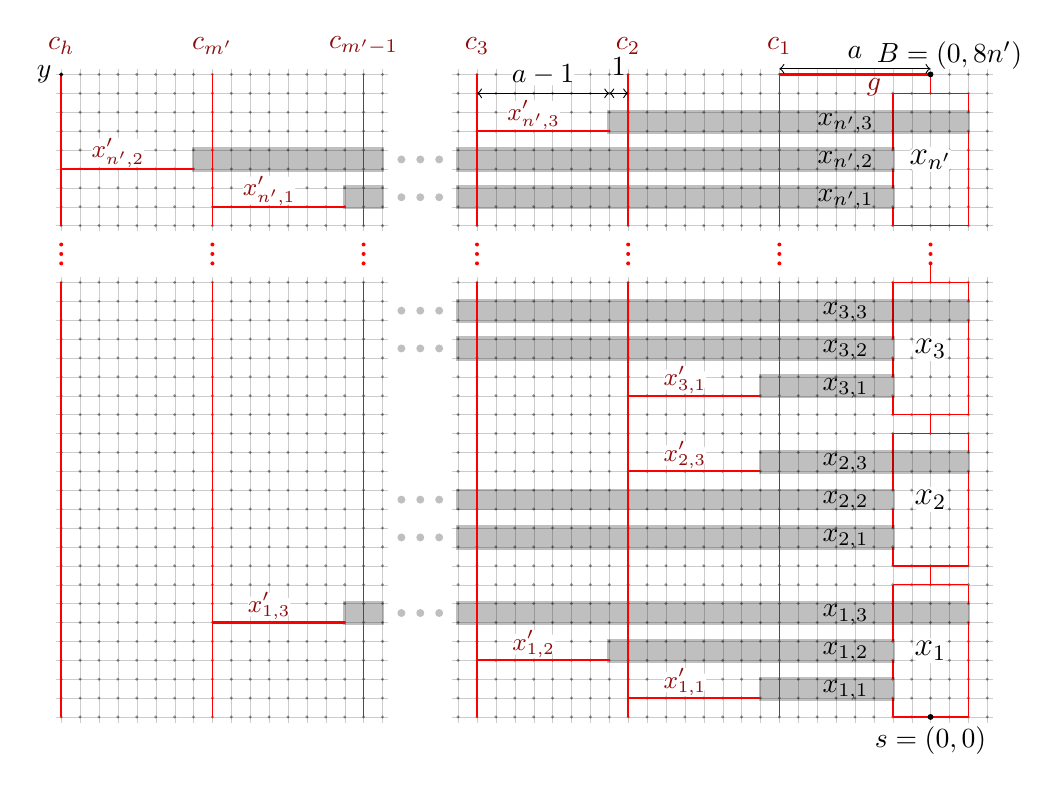
\begin{tikzpicture}[scale=0.24]
\definecolor{dred}{RGB}{143, 11, 11}
\def\wi{0.08}
\def\op{0.2}
\def\pts{2.5pt}

\foreach \x in {-25,...,3} {
\foreach \y in {0,...,23} {
\fill[black, opacity=0.4] (\x, \y) circle (\pts);
}
\draw[black, line width=\wi, opacity=\op] (\x, -0.3) -- (\x, 23.3);
}
\foreach \y in {0,...,23} {
\draw[black, line width=\wi, opacity=\op] (-25.3, \y) -- (3.3, \y);
\draw[black, line width=\wi, opacity=\op] (-46.3, \y) -- (-28.7, \y);
}
\foreach \y in {26,...,34} {
\draw[black, line width=\wi, opacity=\op] (-25.3, \y) -- (3.3, \y);
\draw[black, line width=\wi, opacity=\op] (-46.3, \y) -- (-28.7, \y);
}

\foreach \x in {-25,...,3} {
\foreach \y in {26,...,34} {
\fill[black, opacity=0.4] (\x, \y) circle (\pts);
}
\draw[black, line width=\wi, opacity=\op] (\x, 25.7) -- (\x, 34.3);
}


\foreach \x in {-46,...,-29} {
\foreach \y in {26,...,34} {
\fill[black, opacity=0.4] (\x, \y) circle (\pts);
}
\draw[black, line width=\wi, opacity=\op] (\x, 25.7) -- (\x, 34.3);

}
\foreach \x in {-46,...,-29} {
\foreach \y in {0,...,23} {
\fill[black, opacity=0.4] (\x, \y) circle (\pts);
}
\draw[black, line width=\wi, opacity=\op] (\x, -0.3) -- (\x, 23.3);
}
\draw[red, line width = 0.5669291340000001pt]   (-2, 0) -- (2, 0);
\draw[red, line width = 0.5669291340000001pt]   (-2, 0) -- (-2, 1);
\draw[red, line width = 0.5669291340000001pt]   (-2, 2) -- (-2, 3);
\draw[red, line width = 0.5669291340000001pt]   (-2, 4) -- (-2, 7);
\draw[red, line width = 0.5669291340000001pt]   (2, 0) -- (2, 5);
\draw[red, line width = 0.5669291340000001pt]   (2, 6) -- (2, 7);
\draw[red, line width = 0.5669291340000001pt]   (-2, 7) -- (2, 7);
\draw[red, line width = 0.5669291340000001pt]   (0, 7) -- (0, 8);
\node[fill=white, rounded corners, inner sep=1pt, outer sep=1pt] at (0, 3.5)  {\large $x_1$};
\draw[red, line width = 0.5669291340000001pt]   (-2, 8) -- (2, 8);
\draw[red, line width = 0.5669291340000001pt]   (-2, 8) -- (-2, 9);
\draw[red, line width = 0.5669291340000001pt]   (-2, 10) -- (-2, 11);
\draw[red, line width = 0.5669291340000001pt]   (-2, 12) -- (-2, 15);
\draw[red, line width = 0.5669291340000001pt]   (2, 8) -- (2, 13);
\draw[red, line width = 0.5669291340000001pt]   (2, 14) -- (2, 15);
\draw[red, line width = 0.5669291340000001pt]   (-2, 15) -- (2, 15);
\draw[red, line width = 0.5669291340000001pt]   (0, 15) -- (0, 16);
\node[fill=white, rounded corners, inner sep=1pt, outer sep=1pt] at (0, 11.5)  {\large $x_2$};
\draw[red, line width = 0.5669291340000001pt]   (-2, 16) -- (2, 16);
\draw[red, line width = 0.5669291340000001pt]   (-2, 16) -- (-2, 17);
\draw[red, line width = 0.5669291340000001pt]   (-2, 18) -- (-2, 19);
\draw[red, line width = 0.5669291340000001pt]   (-2, 20) -- (-2, 23);
\draw[red, line width = 0.5669291340000001pt]   (2, 16) -- (2, 21);
\draw[red, line width = 0.5669291340000001pt]   (2, 22) -- (2, 23);
\draw[red, line width = 0.5669291340000001pt]   (-2, 23) -- (2, 23);
\draw[red, line width = 0.5669291340000001pt]   (0, 23) -- (0, 24);
\node[fill=white, rounded corners, inner sep=1pt, outer sep=1pt] at (0, 19.5)  {\large$x_3$};
\draw[red, line width = 0.5669291340000001pt]   (-2, 26) -- (2, 26);
\draw[red, line width = 0.5669291340000001pt]   (-2, 26) -- (-2, 27);
\draw[red, line width = 0.5669291340000001pt]   (-2, 28) -- (-2, 29);
\draw[red, line width = 0.5669291340000001pt]   (-2, 30) -- (-2, 33);
\draw[red, line width = 0.5669291340000001pt]   (2, 26) -- (2, 31);
\draw[red, line width = 0.5669291340000001pt]   (2, 32) -- (2, 33);
\draw[red, line width = 0.5669291340000001pt]   (-2, 33) -- (2, 33);
\draw[red, line width = 0.5669291340000001pt]   (0, 33) -- (0, 34);
\node[fill=white, rounded corners, inner sep=1pt, outer sep=1pt] at (0, 29.5)  {\large $x_{n'}$};
\draw[black, line width = 8.736220474000001pt, opacity=0.25]   (-9.1, 1.5) -- (-1.9, 1.5);
\node at (-4.5, 1.4) { $x_{1, 1}$};
\draw[black, line width = 8.736220474000001pt, opacity=0.25]   (-17.1, 3.5) -- (-1.9, 3.5);
\node at (-4.5, 3.4) { $x_{1, 2}$};
\draw[black, line width = 8.736220474000001pt, opacity=0.25]   (-25.1, 5.5) -- (2.1, 5.5);
\node at (-4.5, 5.4) { $x_{1, 3}$};
\fill[black, opacity=0.25] (-26, 5.5) circle (6pt);
\fill[black, opacity=0.25] (-27, 5.5) circle (6pt);
\fill[black, opacity=0.25] (-28, 5.5) circle (6pt);
\draw[black, line width = 8.736220474000001pt, opacity=0.25]   (-31.1, 5.5) -- (-28.9, 5.5);
\draw[black, line width = 8.736220474000001pt, opacity=0.25]   (-25.1, 9.5) -- (-1.9, 9.5);
\node at (-4.5, 9.4) { $x_{2, 1}$};
\fill[black, opacity=0.25] (-26, 9.5) circle (6pt);
\fill[black, opacity=0.25] (-27, 9.5) circle (6pt);
\fill[black, opacity=0.25] (-28, 9.5) circle (6pt);
\draw[black, line width = 7.836220474000001pt, opacity=0.25]   (-25.1, 11.5) -- (-1.9, 11.5);
\node at (-4.5, 11.4) { $x_{2, 2}$};
\fill[black, opacity=0.25] (-26, 11.5) circle (6pt);
\fill[black, opacity=0.25] (-27, 11.5) circle (6pt);
\fill[black, opacity=0.25] (-28, 11.5) circle (6pt);
\draw[black, line width = 8.736220474000001pt, opacity=0.25]   (-9.1, 13.5) -- (2.1, 13.5);
\node at (-4.5, 13.4) { $x_{2, 3}$};
\draw[black, line width = 8.736220474000001pt, opacity=0.25]   (-9.1, 17.5) -- (-1.9, 17.5);
\node at (-4.5, 17.4) { $x_{3, 1}$};
\draw[black, line width = 8.736220474000001pt, opacity=0.25]   (-25.1, 19.5) -- (-1.9, 19.5);
\node at (-4.5, 19.4) { $x_{3, 2}$};
\fill[black, opacity=0.25] (-26, 19.5) circle (6pt);
\fill[black, opacity=0.25] (-27, 19.5) circle (6pt);
\fill[black, opacity=0.25] (-28, 19.5) circle (6pt);
\draw[black, line width = 8.736220474000001pt, opacity=0.25]   (-25.1, 21.5) -- (2.1, 21.5);
\node at (-4.5, 21.4) { $x_{3, 3}$};
\fill[black, opacity=0.25] (-26, 21.5) circle (6pt);
\fill[black, opacity=0.25] (-27, 21.5) circle (6pt);
\fill[black, opacity=0.25] (-28, 21.5) circle (6pt);
\draw[black, line width = 8.736220474000001pt, opacity=0.25]   (-25.1, 27.5) -- (-1.9, 27.5);
\node at (-4.5, 27.4) { $x_{n', 1}$};
\fill[black, opacity=0.25] (-26, 27.5) circle (6pt);
\fill[black, opacity=0.25] (-27, 27.5) circle (6pt);
\fill[black, opacity=0.25] (-28, 27.5) circle (6pt);
\draw[black, line width = 8.736220474000001pt, opacity=0.25]   (-25.1, 29.5) -- (-1.9, 29.5);
\node at (-4.5, 29.4) { $x_{n', 2}$};
\fill[black, opacity=0.25] (-26, 29.5) circle (6pt);
\fill[black, opacity=0.25] (-27, 29.5) circle (6pt);
\fill[black, opacity=0.25] (-28, 29.5) circle (6pt);
\draw[black, line width = 8.736220474000001pt, opacity=0.25]   (-17.1, 31.5) -- (2.1, 31.5);
\node at (-4.5, 31.4) { $x_{n', 3}$};
% \fill[black, opacity=0.25] (-26, 31.5) circle (6pt);
% \fill[black, opacity=0.25] (-27, 31.5) circle (6pt);
% \fill[black, opacity=0.25] (-28, 31.5) circle (6pt);
\draw[black, line width = 8.736220474000001pt, opacity=0.25]   (-31.1, 27.5) -- (-28.9, 27.5);
\draw[black, line width = 8.736220474000001pt, opacity=0.25]   (-39.1, 29.5) -- (-28.9, 29.5);
\node at (-8, 35.5)  {$\textcolor{dred}{c_1}$};
\draw[red, line width = 0.5669291340000001pt]   (-8, 0) -- (-8, 23);
\draw[red, line width = 0.5669291340000001pt]   (-8, 26) -- (-8, 34);
\fill[red] (-8, 24) circle (3pt);
\fill[red] (-8, 24.5) circle (3pt);
\fill[red] (-8, 25) circle (3pt);
\node at (-16, 35.5)  {$\textcolor{dred}{c_2}$};
\draw[red, line width = 0.5669291340000001pt]   (-16, 0) -- (-16, 23);
\draw[red, line width = 0.5669291340000001pt]   (-16, 26) -- (-16, 34);
\fill[red] (-16, 24) circle (3pt);
\fill[red] (-16, 24.5) circle (3pt);
\fill[red] (-16, 25) circle (3pt);
\node at (-24, 35.5)  {$\textcolor{dred}{c_3}$};
\draw[red, line width = 0.5669291340000001pt]   (-24, 0) -- (-24, 23);
\draw[red, line width = 0.5669291340000001pt]   (-24, 26) -- (-24, 34);
\fill[red] (-24, 24) circle (3pt);
\fill[red] (-24, 24.5) circle (3pt);
\fill[red] (-24, 25) circle (3pt);
\node at (-30, 35.5)  {$\textcolor{dred}{c_{m'-1}}$};
\draw[red, line width = 0.5669291340000001pt]   (-30, 0) -- (-30, 23);
\draw[red, line width = 0.5669291340000001pt]   (-30, 26) -- (-30, 34);
\fill[red] (-30, 24) circle (3pt);
\fill[red] (-30, 24.5) circle (3pt);
\fill[red] (-30, 25) circle (3pt);
\node at (-38, 35.5)  {$\textcolor{dred}{c_{m'}}$};
\draw[red, line width = 0.5669291340000001pt]   (-38, 0) -- (-38, 23);
\draw[red, line width = 0.5669291340000001pt]   (-38, 26) -- (-38, 34);
\fill[red] (-38, 24) circle (3pt);
\fill[red] (-38, 24.5) circle (3pt);
\fill[red] (-38, 25) circle (3pt);
\node at (-46, 35.5)  {$\textcolor{dred}{c_h}$};
\draw[red, line width = 0.5669291340000001pt]   (-46, 0) -- (-46, 23);
\draw[red, line width = 0.5669291340000001pt]   (-46, 26) -- (-46, 34);
\fill[red] (-46, 24) circle (3pt);
\fill[red] (-46, 24.5) circle (3pt);
\fill[red] (-46, 25) circle (3pt);
\fill[red] (0, 24) circle (3pt);
\fill[red] (0, 24.5) circle (3pt);
\fill[red] (0, 25) circle (3pt);
\draw[red, line width = 0.8503937010000002pt]   (-8, 34) -- (0, 34);
\draw[red, line width = 0.8503937010000002pt]   (-16, 1) -- (-9, 1);
\node[fill=white, rounded corners, inner sep=0pt, outer sep=0pt] at (-13, 1.85) { \small $\textcolor{dred}{x_{1, 1}'}$};
\draw[red, line width = 0.8503937010000002pt]   (-16, 13) -- (-9, 13);
\node[fill=white, rounded corners, inner sep=0pt, outer sep=0pt] at (-13, 13.85) { \small $\textcolor{dred}{x_{2, 3}'}$};
\draw[red, line width = 0.8503937010000002pt]   (-16, 17) -- (-9, 17);
\node[fill=white, rounded corners, inner sep=0pt, outer sep=0pt] at (-13, 17.85) { \small $\textcolor{dred}{x_{3, 1}'}$};
\draw[red, line width = 0.8503937010000002pt]   (-24, 3) -- (-17, 3);
\node[fill=white, rounded corners, inner sep=0pt, outer sep=0pt] at (-21, 3.85) { \small $\textcolor{dred}{x_{1, 2}'}$};
\draw[red, line width = 0.8503937010000002pt]   (-24, 31) -- (-17, 31);
\node[fill=white, rounded corners, inner sep=0pt, outer sep=0pt] at (-21, 31.85) { \small $\textcolor{dred}{x_{n', 3}'}$};
\draw[red, line width = 0.8503937010000002pt]   (-38, 5) -- (-31, 5);
\node[fill=white, rounded corners, inner sep=0pt, outer sep=0pt] at (-35, 5.85) { \small $\textcolor{dred}{x_{1, 3}'}$};
\draw[red, line width = 0.8503937010000002pt]   (-38, 27) -- (-31, 27);
\node[fill=white, rounded corners, inner sep=0pt, outer sep=0pt] at (-35, 27.85) { \small $\textcolor{dred}{x_{n', 1}'}$};
\draw[red, line width = 0.8503937010000002pt]   (-46, 29) -- (-39, 29);
\node[fill=white, rounded corners, inner sep=0pt, outer sep=0pt] at (-43, 29.85) { \small $\textcolor{dred}{x_{n', 2}'}$};
%\filldraw (0, -4) circle (2pt);
%\node[left] at (0, -4) {$s=(0, - n^5)$};
\filldraw (0, 0) circle (3.5pt);
\node[below] at (0, 0) {$s = (0, 0)$};
\filldraw (0, 34) circle (3.5pt);
\node[] at (1, 35) {$B = (0, 8n')$};
\filldraw (-46, 34) circle (2pt);
\node[left] at (-46, 34) {$y$};
\draw[<->] (-24, 33) -- (-17, 33) node[midway, above=3pt, fill=white, rounded corners, inner sep=0pt, outer sep=0pt] {$a-1$};
\draw[<->] (-17, 33) -- (-16, 33) node[midway, above=3pt] {$1$};
\draw[<->] (-8, 34.3) -- (0, 34.3) node[midway, above] {$a$};
%\draw[black, line width = 0.5669291340000001pt]   (0, 0) -- (0, -4);
%\node[left] at (0, -2)  {$d$};
\node[fill=white, rounded corners, inner sep=0pt, outer sep=0pt] at (-3, 33.3) {$\textcolor{dred}{g}$};
%\node[fill=white, rounded corners] at (0, 0) {$s$};
\end{tikzpicture}
%[Finished in 0.1s]
%     \caption{}
% \label{fig:grid_2speed}
% \end{figure}

%  Once we can get ride of the delay, in our hardness proof, e can present the following result regarding inapproximability:

% \begin{theorem}
%     For the setting without initial positions it is not possible to approximate DDTGR within any poly(n,k) approximation ratio.
% \end{theorem}
% \todo{review and move proof to Appendix}
% \begin{proof}
%     Observe that in the setting without initial positions an optimal schedule takes time $some-value$, assuming $\phi$ has a feasible assignment. If there does not exist a feasible assignment then a variable agent has to travel from right to left to fill a gap in the variable gadget and also fill a gap in some clause gadget(s). However travelling from right to left with a slow agent takes time $some-larger-value$. Therefore, if we could approximate DDTGR by a ratio of $-ratio-$, then we could solve \textsc{2P1N-3SAT}.
% \end{proof}


% \subsection{NP-Hardness for unit speed drones and arbitrary movement areas} 
% \label{1grid}
% We can adapt the core construction of section \ref{2grid} to achieve similar results for  agents with unit speed and arbitrary movement areas, though some adjustments are necessary. The construction in \ref{2grid} only works if the speed of the fast agents exceeds that of the slower (variable) agents. 
% Nevertheless, the flexibility of arbitrary movement areas allows us to cope with that.  Since we are not confined to rectangular paths, we can simulate slower speeds by requiring agents to take detours. The movement areas of the variable agents are depicted in Figure \ref{fig:grid_1speed}. By setting the vertical spacing of agents $x_{i,1},x_{i,2}$ and $x_{i,3}$ to 2, we can replicate the same speeds used in the construction for two speeds and rectangular movement areas. Therefore, the results are transferable, and we can state our result below. Due to space limitations, the proof is omitted. % We will not prove it but argue that the proof can be done analogously to the proof of Theorem \ref{thm:grid_2speed} in Appendix \ref{sec:appendixDDTGRproof}.

%\thmgridspeed* 

% \begin{proof}
%     We proof the theorem by arguing that there exist feasible values for $a$ and $b$ to model the case for the proof of Theorem \ref{thm:grid_2speed}. Note that the size of the grid does also not significantly grow. \todo{is that actually true, I dont know the values}
% \end{proof}


% \begin{theorem}
%     For the setting without initial positions it is not possible to approximate DDTG within any poly(n,k) approximation ratio.
% \end{theorem}
% \vspace{-2mm}
% \begin{figure}[h]
%     \centering
%     \input{grid_1speed}
%     \caption{A close up on a variable gadget (right side) as well as a clause gadget (left side)} for the DDTGU instance. The general construction does not differ from the DDTGR case. Due to the relaxation in movement areas, we make the variable agents $x_{i,1},x_{i,2},x_{i,3}$ move via large detours when traveling horizontally, somewhat introducing a second slow speed. Note that although we use different colors the agents' speeds are equal. 
% \label{fig:grid_1speed}
% \end{figure}

